\chapter{Desenvolvimento: MeuPetAqui}

O MeuPetAqui\footnote{MeuPetAqui - Disponível em: http://vps45018.publiccloud.com.br/app/}  é uma rede social que tem como objetivo ajudar ONGs e protetores de animais de Vitória da Conquista, além de promover e incentivar o cuidado com os animais de estimação. Para desenvolvê-la, optou-se pela tecnologia de serviço web para tornar o acesso fácil e rápido por meio de desktops, smartphones e outros dispositivos com conexão à internet e navegadores web. A rede social é composta por dois tipos de usuários: os que possuem animais de estimação ou gostam de animais e os representantes de ONGs e protetores de animais. Os usuários podem criar perfis específicos para cada um dos seus pets, com postagens contendo imagens e relatos do dia a dia de seus companheiros. Eles também podem acompanhar as postagens de outros usuários, reagir com comentários e curtidas, criando assim um vínculo de amizade entre cuidadores.

A plataforma oferece um serviço completo de divulgação de ocorrências, que permite aos usuários informar sua rede de contatos e os usuários do sistema sobre pets perdidos, encontrados, para adoção e animais que precisam de tratamento veterinário. Além disso, o sistema disponibiliza o serviço RGA (Registro Geral Animal), uma ferramenta que facilita a identificação do tutor ou busca de informações do pet. E para auxiliar no controle de vacinas e medicamentos, é disponibilizada uma cartilha de vacinação. Ainda, é importante ressaltar que a plataforma conta com uma interface amigável e de fácil utilização, seguindo padrões visuais presentes em outras redes sociais, facilitando a adaptação ao seu uso o que proporciona uma experiência agradável aos usuários. Esses recursos foram desenvolvidos visando atender às necessidades e demandas dos usuários, além de proporcionar uma solução prática e eficiente para o cuidado com os animais de estimação.

A seguir são apresentados os detalhes do MeuPetAqui. Na Seção 5.1 é apresentada a criação de Posts, o feed e a interação com os posts na plataforma. Em seguinda, na Seção 5.2 é demonstrado o perfil destinado ao usuário do sistema e a sua configuração. Na Seção 5.3 temos a galeria de fotos do usuário. Seguindo para a Seção 5.4 é mostrado os pets do usuário. Na Seção 5.5 é tratado o cadastro dos pets. Na Seção 5.6 é tratado o perfil do pet, sua configuração, o RGA e o Cartão de Vacinas. Na Seção 5.7 temos a geração de alertas e o feed de alertas. Seguindo, na Seção 5.8 é demonstrado o processo de rastreamento de pets. Na Seção 5.9 é exibida o guia de páginas de pets cadastrados e geridos por ONGs.

\newpage

\section{Posts}
O MeuPetAqui é uma plataforma que se baseia em outras redes sociais, tendo como uma de suas principais atividades a criação de postagens. Através dessa função, o usuário pode gerar conteúdo personalizado, adicionando imagens e vinculando seus pets aos posts.

Ao criar uma postagem, o usuário pode selecionar a imagem que deseja anexar à publicação, tornando-a mais atraente visualmente. Além disso, é possível adicionar os pets associados àquela postagem. Dessa forma, ao entrar no perfil de um pet específico, todas as imagens postadas e relacionadas a ele estarão presentes na galeria de imagens do perfil.

Essa função do MeuPetAqui permite que os usuários compartilhem experiências, dicas e histórias sobre seus animais de estimação de maneira personalizada, tornando a plataforma uma fonte valiosa de informações e conexões para os amantes de pets. (Figura \ref{fig:CriaçãodePosts}).


\begin{figure}[htb]
     \centering
     \FonteFig{Elaborado pelo autor}
     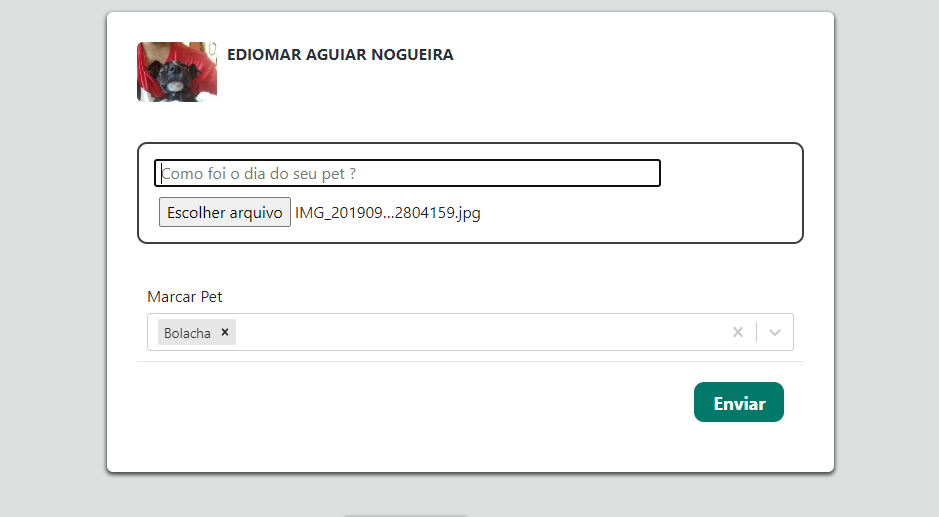
\includegraphics[width=14cm]{arquivos/Figuras/image27.png}
     \caption{Criação de Posts}
     \label{fig:CriaçãodePosts}
\end{figure}

\newpage
\subsection{Feed de Posts}
\label{subsec:FeedPosts}
O feed de postagens é o local onde o usuário pode visualizar suas próprias postagens e as postagens das pessoas que ele segue ou tem amizade dentro da plataforma. A listagem dos posts é organizada por ordem cronológica, do mais recente ao mais antigo, independentemente de quem tenha feito a publicação. (Figura \ref{fig:FeedDePosts}).

\begin{figure}[htb]
     \centering
     \FonteFig{Elaborado pelo autor}
     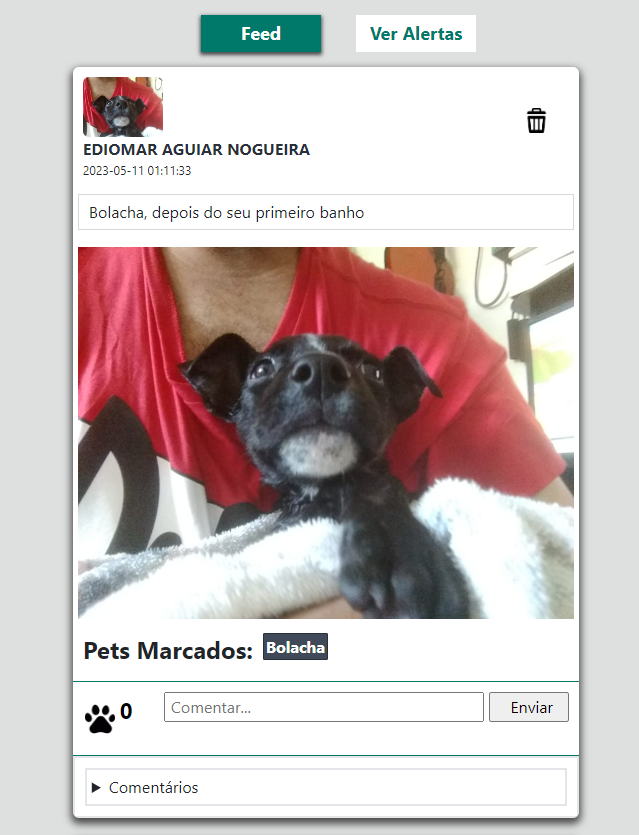
\includegraphics[width=10cm]{arquivos/Figuras/image17.png}
     \caption{Feed de Posts}
     \label{fig:FeedDePosts}
\end{figure}

Inicialmente, o feed exibe até 6 posts. Ao chegar ao final da página, o usuário pode solicitar o carregamento de mais 6 posts, e assim sucessivamente enquanto houver conteúdo para ser carregado. Essa abordagem de carregamento por demanda ajuda a tornar a experiência de navegação mais fluida e evita sobrecarregar a página com uma grande quantidade de informações de uma só vez.

Os posts podem conter mensagens, imagens e marcação de pets, mas a presença da foto, nome do autor e data e hora são obrigatórias. Ao clicar no nome do criador do post ou em um pet marcado na publicação, o usuário é redirecionado para a página do perfil do criador ou do pet.

O usuário que criou o post tem a opção de excluir a publicação ao visualizá-la. Isso proporciona mais controle e autonomia para o usuário gerenciar o seu conteúdo na plataforma.

\subsection{Interação aos posts}
Os usuários podem interagir com os posts através de curtidas, indicando que gostaram do conteúdo, ou com comentários, permitindo uma comunicação mais direta e interativa. Cada comentário possui a data de criação, o nome e a foto do autor. Ao clicar no nome do autor, o usuário é direcionado para a página de perfil daquele usuário que criou o comentário. Isso incentiva uma maior interação entre os usuários e torna a experiência na plataforma mais dinâmica e envolvente. (Figura \ref{fig:InteraçãoAosPosts}).

\begin{figure}[htb]
     \centering
     \FonteFig{Elaborado pelo autor}
     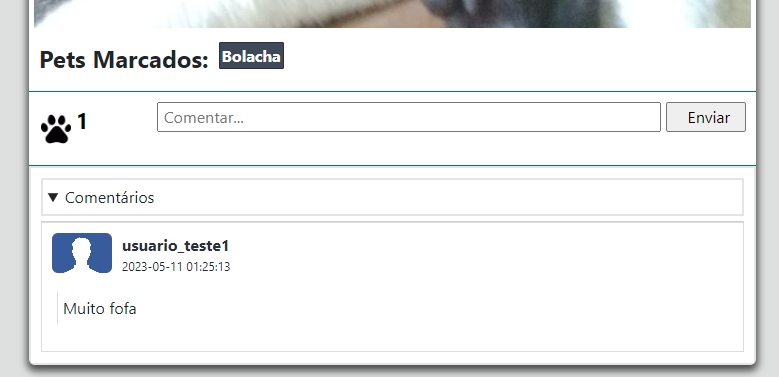
\includegraphics[width=12cm]{arquivos/Figuras/image11.png}
     \caption{Interação aos Posts}
     \label{fig:InteraçãoAosPosts}
\end{figure}

\begin{table}[htbp]
\centering
\renewcommand{\arraystretch}{1.5}
\begin{tabular}{|c|>{\centering\arraybackslash}m{6cm}|c|}
\hline
\textbf{Link} & \textbf{QR Code} \\
\hline
\href{https://drive.google.com/file/d/1QR-FYXyBn2FoYs8XX4q8F1Ivxa3LxWyp/view?usp=drive_link}{Armazenamento em Google Drive} & 
\includegraphics[width=3.5cm]{arquivos/ImgLinks/posts.png} \\
\hline
\end{tabular}
\caption*{Vídeo de demonstração dos posts - Fonte: Próprio autor}
\end{table}

\newpage
\section{Vinculo entre usuários}
\label{sec:VinculoEntreUsuarios}
O MeuPetAqui disponibiliza a funcionalidade de seguir outros usuários, permitindo o acesso às suas postagens. Na página inicial, no menu esquerdo, é exibida uma lista de usuários recomendados para seguir. Essa recomendação é baseada na proximidade geográfica em relação ao usuário, utilizando as informações de localização fornecidas durante o cadastro. Os usuários mais próximos são exibidos em posições superiores na lista. (Figura \ref{fig:UsuariosProximos}).

\begin{figure}[htb]
     \centering
     \FonteFig{Elaborado pelo autor}
     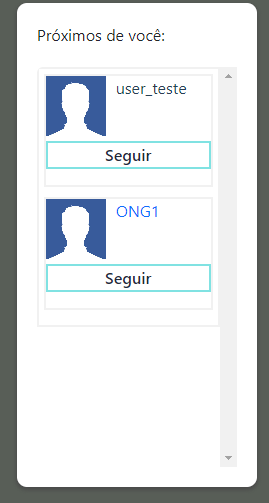
\includegraphics[width=6cm]{arquivos/Figuras/usuarioproximo.png}
     \caption{Usuários próximos para seguir}
     \label{fig:UsuariosProximos}
\end{figure}

Ao acessar o perfil de um usuário, são exibidas informações sobre suas conexões sociais. Essas informações incluem a quantidade de amigos, que representa a soma das pessoas que o usuário segue e também são seguidas por ele. Além disso, são apresentadas a quantidade de seguidores, que indica o número de usuários que seguem o perfil do usuário, e a quantidade de perfis seguidos pelo usuário, que indica a quantidade de usuários que o usuário está seguindo. Essas métricas fornecem uma visão abrangente das interações sociais do usuário no sistema, destacando seus amigos, seguidores e os perfis que ele segue. (Figura \ref{fig:vinculacaoComUsuarios}).

\begin{figure}[htb]
     \centering
     \FonteFig{Elaborado pelo autor}
     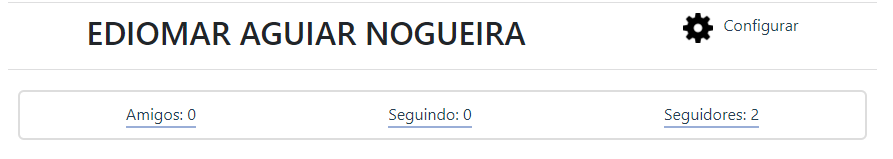
\includegraphics[width=10cm]{arquivos/Figuras/vinculados.png}
     \caption{Vinculação com outros usuários}
     \label{fig:vinculacaoComUsuarios}
\end{figure}

Ao clicar em uma das categorias de vínculo, o usuário será direcionado para uma página específica de gerenciamento das suas conexões. Nessa página, ele terá acesso a uma listagem dos perfis que estão vinculados a ele na respectiva categoria selecionada. Essa funcionalidade permite ao usuário visualizar e gerenciar de forma organizada as suas conexões, facilitando a interação com os perfis vinculados. (Figura \ref{fig:amigosSeguidoresSeguindo}).\\

\begin{figure}[htb]
     \centering
     \FonteFig{Elaborado pelo autor}
     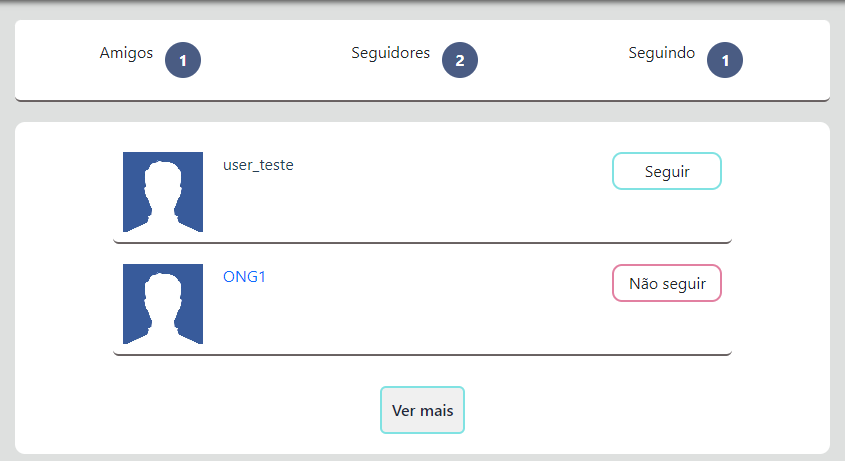
\includegraphics[width=12cm]{arquivos/Figuras/amigosSeguidoresSeguindo.png}
     \caption{Amigos, Seguidores, Seguindo}
     \label{fig:amigosSeguidoresSeguindo}
\end{figure}

\begin{table}[htbp]
\centering
\renewcommand{\arraystretch}{1.5}
\begin{tabular}{|c|>{\centering\arraybackslash}m{6cm}|c|}
\hline
\textbf{Link} & \textbf{QR Code} \\
\hline
\href{https://drive.google.com/file/d/1_f2zeal7lgCEX0xUcvcWqX4u0Sg0Nmqa/view?usp=drive_link}{Armazenamento em Google Drive} & 
\includegraphics[width=3.5cm]{arquivos/ImgLinks/vinculo.png} \\
\hline
\end{tabular}
\caption*{Vídeo sobre vínculo entre usuários - Fonte: Próprio autor}
\end{table}

\newpage
\section{Perfil de usuário}
\label{sec:PerfilDeUsuario}
O perfil do usuário é a página do sistema que reúne todas as informações pessoais do usuário. Essa página apresenta funcionalidades como a personalização da imagem de capa, que permite que o usuário escolha uma imagem que reflita seu carinho pelo seu pet ou sua personalidade. Além disso, é possível visualizar o número de seguidores, quantos são seguidos e seguidores mútuos, o que permite ao usuário ter uma noção do seu alcance na plataforma.

Uma característica importante dessa página é a possibilidade de conectar outras redes sociais ao sistema. Quando o usuário informa suas outras redes sociais, o sistema disponibiliza links diretos para essas páginas, o que facilita a conexão entre as diferentes plataformas, função especialmente importante para ONGs e Protetores de animais, por colaborar com a divulgação de seus trabalhos.

Outra funcionalidade crucial é a disponibilidade de rastreamento de animais de estimação. Quando um usuário cadastra sua cidade, bairro e rua, o sistema passa a disponibilizar o rastreamento de seus animais de estimação pela plataforma. Essa funcionalidade é extremamente útil em casos de animais desaparecidos, ajudando o usuário a localizá-los com mais facilidade.

\newpage
Em resumo, o perfil do usuário é uma das principais páginas no sistema que reúne todas as informações do usuário e oferece diversas funcionalidades, como personalização de imagem de capa, conexão com outras redes sociais e rastreamento de animais de estimação. Essas funcionalidades são de grande utilidade para os usuários e podem tornar a experiência na plataforma ainda mais agradável e útil. (Figura \ref{fig:PerfilDoUsuário}).


\begin{figure}[htb]
     \centering
     \FonteFig{Elaborado pelo autor}
     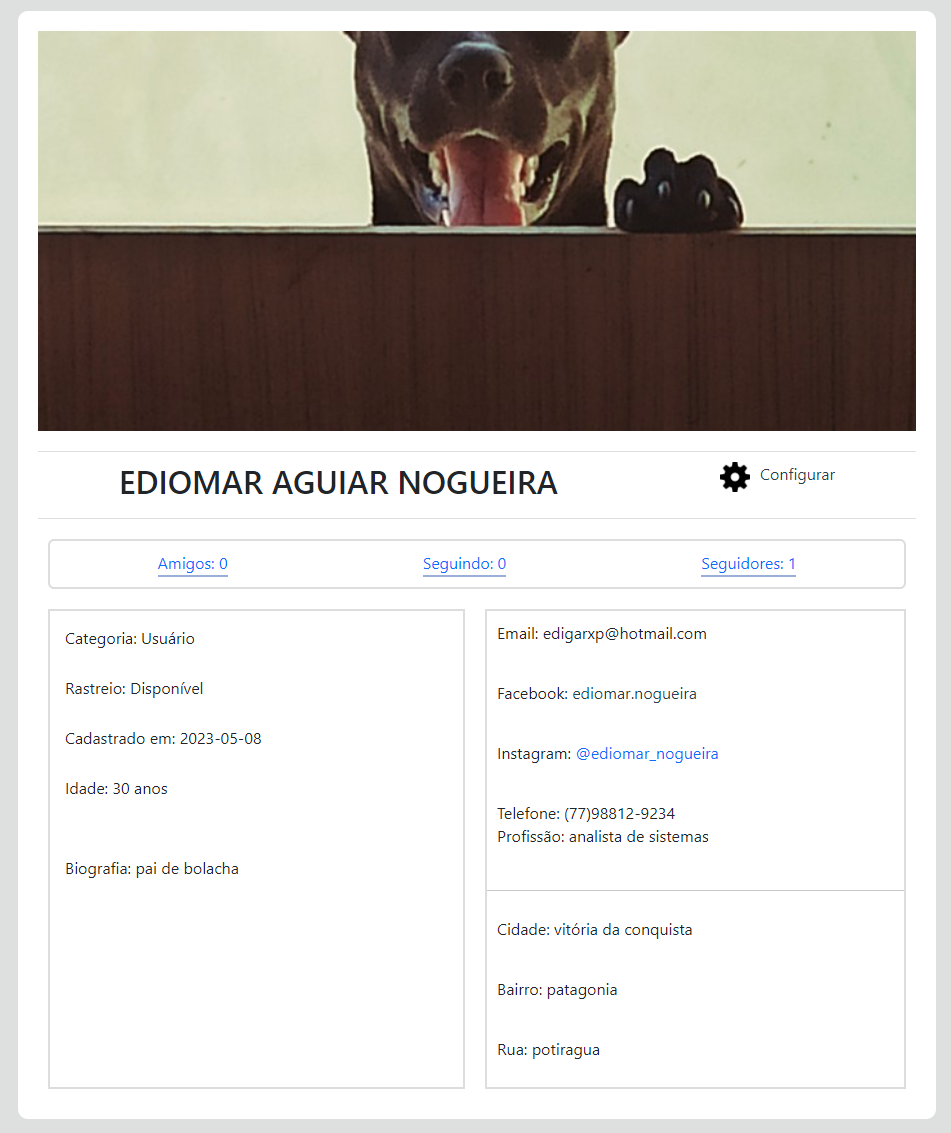
\includegraphics[width=14cm]{arquivos/Figuras/image12.png}
     \caption{Perfil do Usuário}
     \label{fig:PerfilDoUsuário}
\end{figure}

\newpage
\subsection{Configurar Perfil}
O acesso às configurações de perfil de usuário está na página de perfil, nesta seção da plataforma o usuário pode revisar e editar as suas informações. Ao criar um perfil no MeuPetAqui algumas informações não são informadas no momento de cadastro, o usuário deve acessar as configurações de perfil e atualizar seus dados, dentre as informações pedidas, a de maior relevância é referente a sua localização, com base na sua cidade, bairro e rua/avenida, o sistema registra as coordenadas próximas a essas referências e com base nestas coordenadas pode contribuir para o rastreio de seu pet em um possível desaparecimento do mesmo. 

Na plataforma MeuPetAqui, a opção de configurações de perfil do usuário estão localizadas na página de perfil do usuário. Nestas configurações, o usuário pode revisar e editar suas informações pessoais a qualquer momento.

Ao criar um perfil na plataforma, é possível que algumas informações não sejam fornecidas durante o cadastro. Nesses casos, o usuário pode acessar as configurações de perfil para atualizar esses dados. É importante destacar que uma das informações mais relevantes para o usuário inserir é a sua localização, incluindo a cidade, bairro e rua/avenida onde reside. Ao fornecer as informações de sua localidade, o sistema registra as coordenadas próximas a essas referências e, com base nelas, pode auxiliar no rastreamento de animais de estimação em caso de desaparecimento. Isso significa que, em situações críticas, como quando o pet foge ou se perde, o usuário pode contar com o apoio da plataforma para ajudá-lo a encontrar seu animal de estimação.

\newpage
Em resumo, as configurações de perfil do usuário no MeuPetAqui permitem que o usuário revise e atualize suas informações pessoais, incluindo a sua localização. Ao fornecer informações precisas, o sistema pode ajudar o usuário a rastrear seu animal de estimação em caso de desaparecimento, oferecendo uma funcionalidade importante e valiosa para os usuários da plataforma. (Figura \ref{fig:FormulárioCPerfilUsuário}).


\begin{figure}[htb]
     \centering
     \FonteFig{Elaborado pelo autor}
     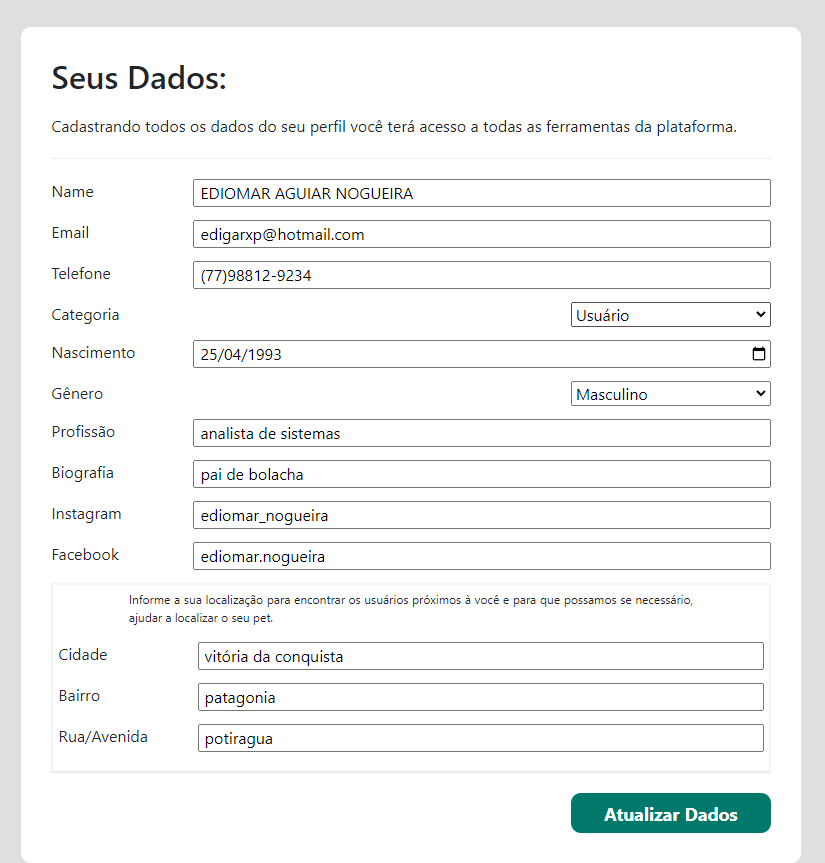
\includegraphics[width=14cm]{arquivos/Figuras/image25.png}
     \caption{Formulário de Configuração do Perfil de Usuário}
     \label{fig:FormulárioCPerfilUsuário}
\end{figure}

Além de permitir que o usuário atualize suas informações pessoais, as configurações de perfil na plataforma MeuPetAqui também oferecem uma funcionalidade de personalização da página do usuário.

Essa personalização permite que o usuário adapte a página de perfil de acordo com suas preferências, personalidade e estilo de vida, além de expressar seu amor pelo seu animal de estimação. Nessa página, o usuário pode fazer alterações na imagem de capa e na imagem de perfil, escolhendo imagens que reflitam sua personalidade e a relação com seu pet.

Em resumo, as configurações de perfil do usuário na plataforma MeuPetAqui permitem que o usuário personalize sua página de perfil, fazendo alterações na imagem de capa e imagem de perfil. Essa funcionalidade de personalização é importante porque permite que o usuário expresse sua personalidade e amor pelo seu pet, tornando a experiência na plataforma ainda mais agradável e personalizada. (Figura \ref{fig:AltDeCapaImagemPerfilUsuário}).

\begin{figure}[htb]
     \centering
     \FonteFig{Elaborado pelo autor}
     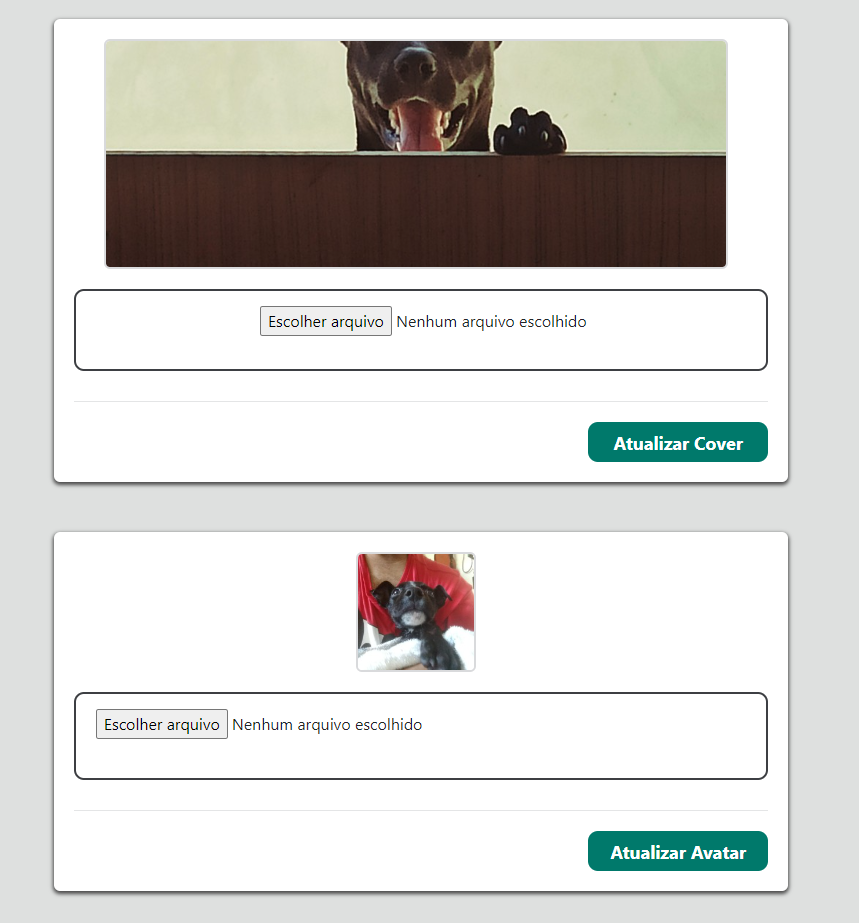
\includegraphics[width=10cm]{arquivos/Figuras/image22.png}
     \caption{Alteração de Capa e Imagem de Perfil de Usuário}
     \label{fig:AltDeCapaImagemPerfilUsuário}
\end{figure}

\begin{table}[htbp]
\centering
\renewcommand{\arraystretch}{1.5}
\begin{tabular}{|c|>{\centering\arraybackslash}m{6cm}|c|}
\hline
\textbf{Link} & \textbf{QR Code} \\
\hline
\href{https://drive.google.com/file/d/19kmkY3OLrkkcErTuMwM3Cx5TxKMiL3cM/view?usp=drive_link}{Armazenamento em Google Drive} & 
\includegraphics[width=3.5cm]{arquivos/ImgLinks/perfilUser.png} \\
\hline
\end{tabular}
\caption*{Vídeo sobre perfil de usuário - Fonte: Próprio autor}
\end{table}

\newpage
\section{Galeria de Fotos}
\label{sec:GaleriaDeFotos}
No MeuPetAqui, existem duas galerias de imagens disponíveis para os usuários. A primeira galeria consiste em todas as fotos postadas pelo usuário, incluindo as fotos com e sem pets marcados. A segunda galeria de fotos está localizada no perfil do pet e contém apenas as fotos onde o pet foi marcado. Se um pet foi marcado em uma foto postada pelo usuário, essa foto aparecerá na galeria de fotos do perfil daquele pet. Para acessar essas galerias de imagens, basta clicar na guia "Galeria de fotos" no menu à esquerda da plataforma ou no perfil do pet, logo abaixo das informações dele. (Figura \ref{fig:GaleriaDeFotosUsuário}).

\begin{figure}[htb]
     \centering
     \FonteFig{Elaborado pelo autor}
     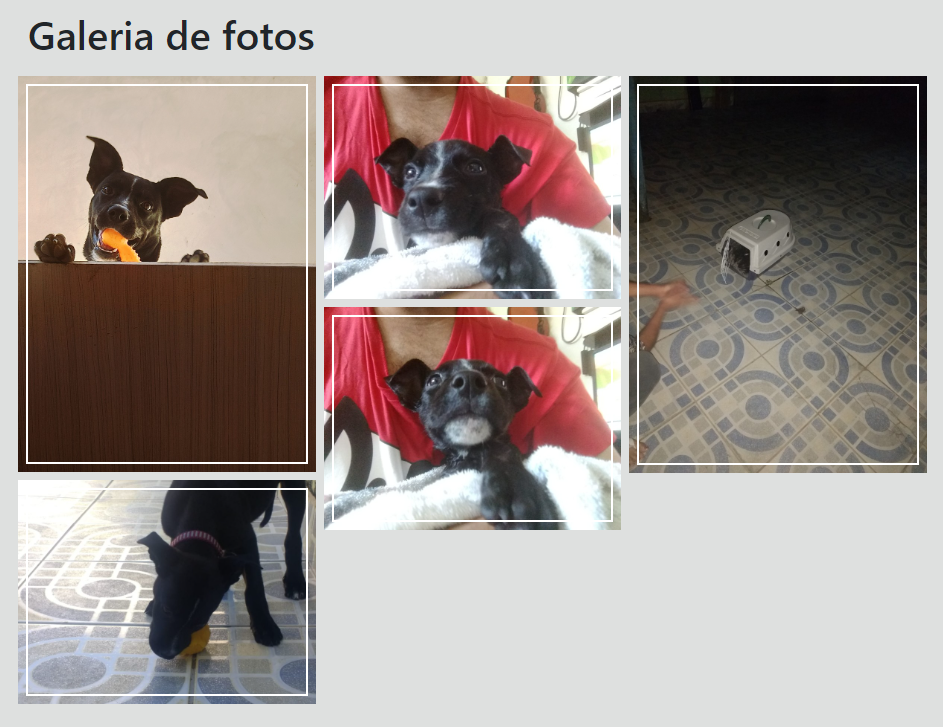
\includegraphics[width=12cm]{arquivos/Figuras/image2.png}
     \caption{Galeria de Fotos}
     \label{fig:GaleriaDeFotosUsuário}
\end{figure}

\begin{table}[htbp]
\centering
\renewcommand{\arraystretch}{1.5}
\begin{tabular}{|c|>{\centering\arraybackslash}m{6cm}|c|}
\hline
\textbf{Link} & \textbf{QR Code} \\
\hline
\href{https://drive.google.com/file/d/1v1G_Ykho823LDGSGFYSppBE6IkCKUW__/view?usp=drive_link}{Armazenamento em Google Drive} & 
\includegraphics[width=3.5cm]{arquivos/ImgLinks/galeriaDeFotos.png} \\
\hline
\end{tabular}
\caption*{Vídeo sobre galeria de fotos do usuário - Fonte: Próprio autor}
\end{table}

\newpage
\section{Pets}
No MeuPetAqui, o usuário tem a possibilidade de criar perfis para cada um de seus pets. Esses perfis são exibidos na guia "Pets", que é o mesmo local onde o usuário pode adicionar um novo pet. Os animais cadastrados são organizados de acordo com a situação informada durante o cadastro, podendo ser separados em: "Meu Pet", "Pet para Adoção", "Pet Desaparecido" e "Encontrei este Pet".

Dessa forma, o usuário pode gerenciar facilmente os perfis dos seus pets na plataforma e manter as informações atualizadas de cada animal. A opção de separar os animais por situação facilita a busca por informações específicas, permitindo que o usuário encontre rapidamente o que procura. Este recurso pode ser útil tanto para os proprietários de pets quanto para aqueles que estão procurando adotar ou ajudar animais perdidos ou encontrados. (Figura \ref{fig:PerfisDePets}).

\begin{figure}[htb]
     \centering
     \FonteFig{Elaborado pelo autor}
     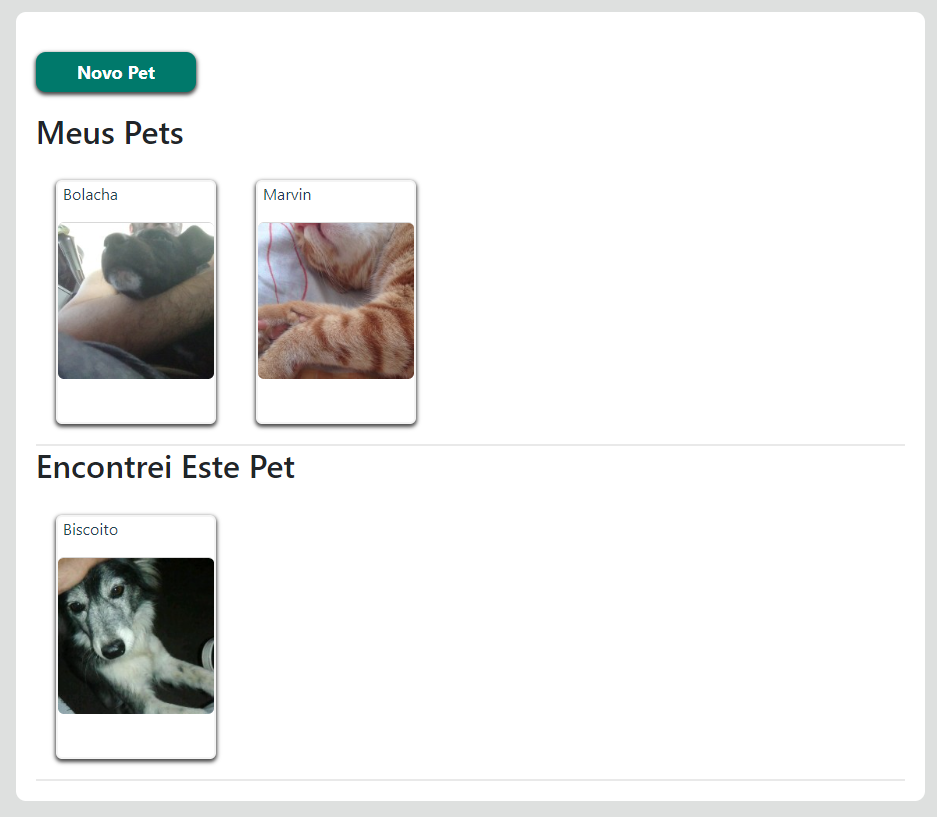
\includegraphics[width=14cm]{arquivos/Figuras/image13.png}
     \caption{Perfis de Pets}
     \label{fig:PerfisDePets}
\end{figure}

\newpage
\section{Cadastro de Pet}
Na página de exibição dos pets do usuário, a guia "Novo Pet" permite que o usuário adicione um novo animal. Ao clicar nesta guia, é exibido um formulário simples para cadastro do pet, que requer informações como nome, espécie, data de nascimento (para estimativa de idade) e a situação em que o pet se encontra, podendo ser: pet do usuário, pet para adoção, pet perdido ou pet encontrado.

Além disso, em perfis de usuário do tipo ONG, há a opção adicional de cadastrar pets que estão em tratamento, indicando que o animal necessita de contribuições para custear o tratamento. Essa opção é uma forma de ajudar animais que precisam de cuidados especiais e que podem não ter um proprietário para arcar com os custos de tratamento. Com essa funcionalidade, a plataforma possibilita que usuários possam auxiliar na recuperação desses animais e fazer a diferença na vida deles. (Figura \ref{fig:CadastroDePets}).

\begin{figure}[htb]
     \centering
     \FonteFig{Elaborado pelo autor}
     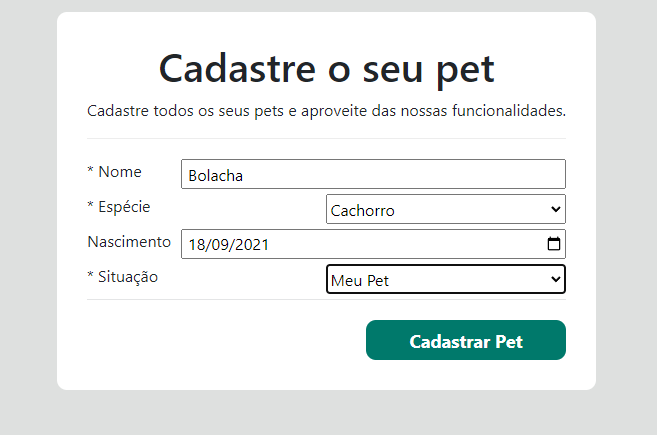
\includegraphics[width=14cm]{arquivos/Figuras/image24.png}
     \caption{Cadastro de Pets}
     \label{fig:CadastroDePets}
\end{figure}

\newpage
\section{Perfil do Pet}

No perfil de Pet, assim como no perfil de usuário, é possível personalizar a página do animal para que ela reflita sua personalidade e características. Isso inclui a opção de alterar a capa e a foto de perfil do animal, deixando a página com uma aparência única e exclusiva. Além disso, logo no início da página do pet, há a opção de configurar o perfil do animal, onde o proprietário pode preencher um formulário com mais informações sobre seu animal de estimação. (Figura \ref{fig:PerfilDoPets}).

\begin{figure}[htb]
     \centering
     \FonteFig{Elaborado pelo autor}
     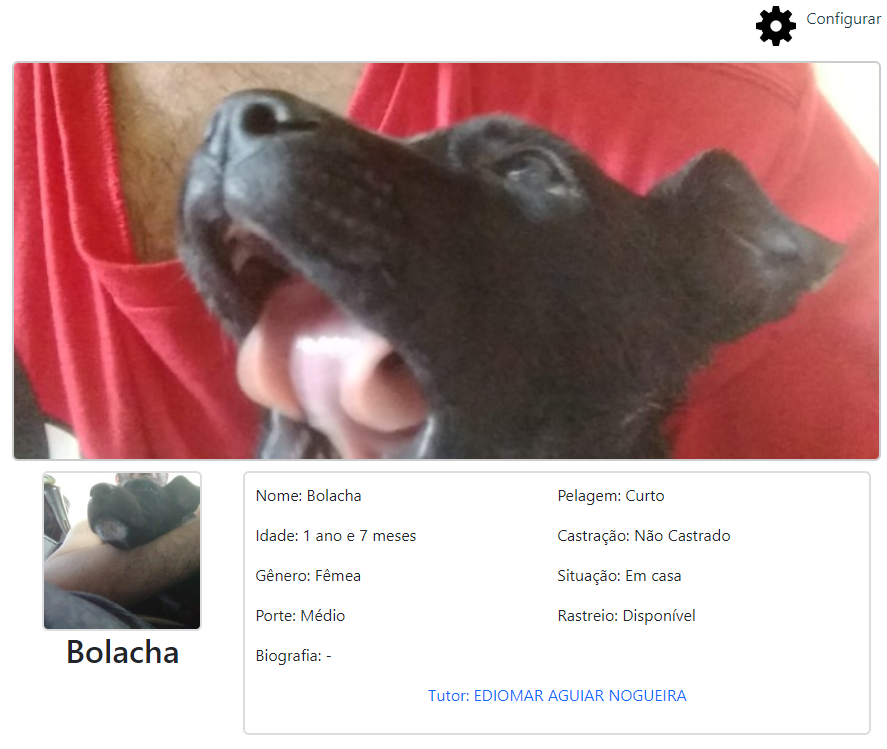
\includegraphics[width=14cm]{arquivos/Figuras/image5.png}
     \caption{Perfil do Pets}
     \label{fig:PerfilDoPets}
\end{figure}

O perfil do pet, conforme exemplificado na Figura \ref{fig:PerfisDePets}, apresenta ao usuário todas as informações cadastradas sobre o animal. Isso inclui a possibilidade de rastreamento do pet, conforme explicado na seção \ref{sec:VinculoEntreUsuarios} sobre o Perfil de Usuário deste trabalho, bem como a identificação do tutor ou ONG responsável pelo cadastro do animal, com um link para o perfil do responsável.
\newpage
Essas informações são extremamente importantes para garantir a segurança e bem-estar do animal, bem como para facilitar a comunicação entre os usuários da plataforma. Com o recurso de rastreamento, é possível localizar rapidamente um animal perdido ou desaparecido e informar o proprietário ou a ONG responsável pelo cadastro. Além disso, a identificação do tutor ou ONG é essencial para que os usuários possam entrar em contato em caso de dúvidas, solicitações ou adoção do animal.

Dessa forma, o perfil do pet é uma parte fundamental da plataforma, permitindo que os usuários visualizem e compartilhem informações sobre seus animais de estimação, facilitando a interação entre os proprietários e a comunidade de animais de estimação.

No perfil do Pet, há outras funcionalidades importantes que merecem destaque, tais como a possibilidade de gerar alertas, acessar a galeria de fotos do animal,como exemplificado na seção \ref{sec:GaleriaDeFotos} sobre Galerias de Fotos, bem como visualizar o RGA (Registro Geral de Animais) e o Cartão de Vacinas do pet. No decorrer deste trabalho, são apresentados exemplos detalhados de como essas funcionalidades podem ser utilizadas e quais são seus benefícios para os usuários da plataforma MeuPetAqui.

\newpage
\subsection{Configurar Perfil do Pet}
De maneira similar ao que foi explicado na seção \ref{sec:PerfilDeUsuario} sobre a Configuração de Perfil de Usuário, a página de configuração de informações do pet também permite ao usuário inserir uma nova capa e imagem de perfil para personalizar o ambiente de acordo com as características do animal. (Figura \ref{fig:EdiçãoCapaFotoPerfilPet}).

\begin{figure}[htb]
     \centering
     \FonteFig{Elaborado pelo autor}
     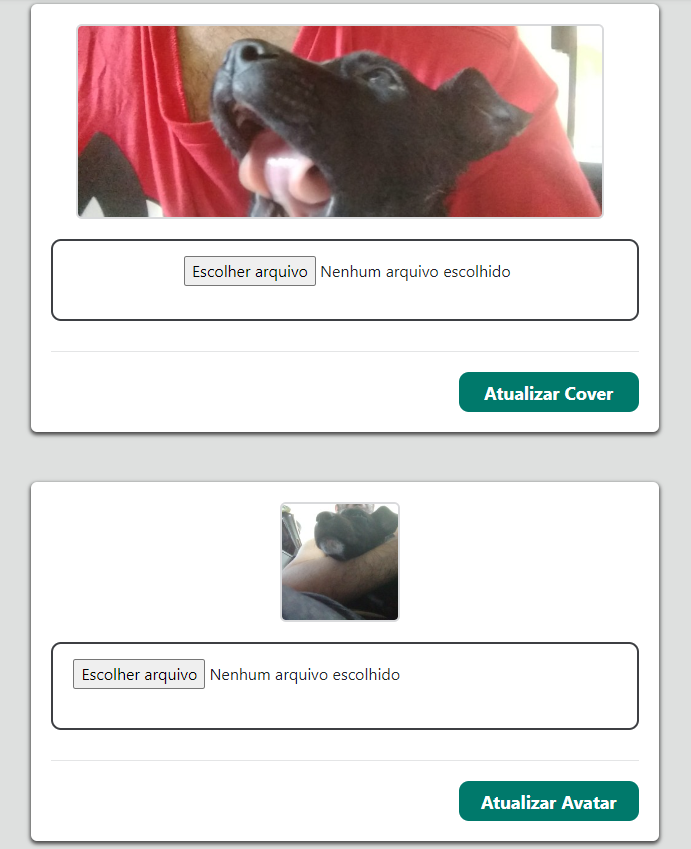
\includegraphics[width=12cm]{arquivos/Figuras/image26.png}
     \caption{Atualização de capa e foto de perfil do pet}
     \label{fig:EdiçãoCapaFotoPerfilPet}
\end{figure}

Na página de configuração dos dados do pet, o usuário tem a possibilidade de informar ou atualizar diversas informações sobre o animal. Dentre elas, é possível definir o nome do pet, a raça, data de nascimento, biografia, status de castração, gênero, espécie, porte, pelagem e situação do pet.

Essa funcionalidade é essencial para que os usuários possam manter as informações do pet atualizadas e compartilhar detalhes importantes sobre o animal com outros usuários da plataforma. Através dessas informações, é possível encontrar animais com características específicas, saber se um pet está disponível para adoção ou encontrar um animal desaparecido. É importante destacar que, em perfis do tipo ONG, há uma opção adicional de informar que um pet está em tratamento, o que permite que a ONG receba contribuições para ajudar no custeio do tratamento do animal. (Figura \ref{fig:ConfigurarDadosPerfilPet}).

\begin{figure}[htb]
     \centering
     \FonteFig{Elaborado pelo autor}
     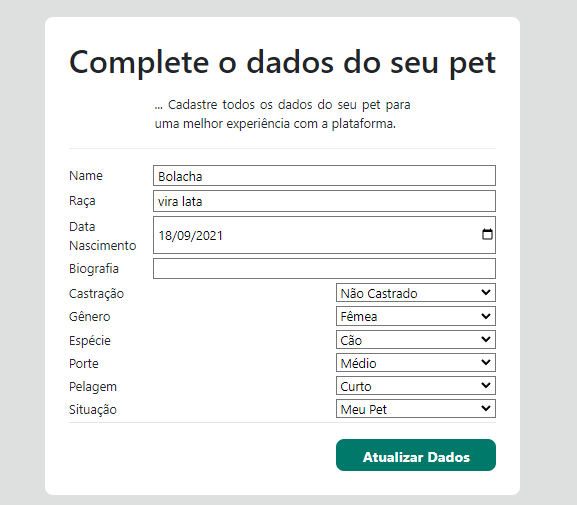
\includegraphics[width=12cm]{arquivos/Figuras/image9.png}
     \caption{Atualização de dados do pet}
     \label{fig:ConfigurarDadosPerfilPet}
\end{figure}

\begin{table}[htbp]
\centering
\renewcommand{\arraystretch}{1.5}
\begin{tabular}{|c|>{\centering\arraybackslash}m{6cm}|c|}
\hline
\textbf{Link} & \textbf{QR Code} \\
\hline
\href{https://drive.google.com/file/d/1UlXozzkAb4PsnaElhlGWawhkKrsX8MIv/view?usp=drive_link}{Armazenamento em Google Drive} & 
\includegraphics[width=3.5cm]{arquivos/ImgLinks/perfilPet.png} \\
\hline
\end{tabular}
\caption*{Vídeo sobre perfil do pet - Fonte: Próprio autor}
\end{table}

\newpage
\subsection{RGA}
Em algumas cidades do Brasil, como é o caso de São Paulo, de acordo com informações obtidas no site da Capital de São Paulo, \citeonline{CapitalSP}, é possível emitir o Registro Geral Animal (RGA) por meio do Centro de Controle de Zoonoses (\gls{CCZ}). Esse documento, similar ao Registro Geral (\gls{RG}) utilizado por humanos, tem como finalidade fornecer uma identificação única para cães e gatos, facilitando o controle de zoonoses e auxiliando na localização de pets desaparecidos.

No MeuPetAqui, embora o RGA não tenha validade legal, sua funcionalidade é similar à aplicada pela prefeitura de São Paulo. Ao cadastrar um pet, o usuário cria um RGA com informações como o nome, espécie, raça, sexo e nome do tutor. O RGA também contém um QRcode\footnote{QRcode - (Quick Response Code) ou “Código de Resposta Rápida”, se trata de uma variação mais moderna do código de barras que pode ser lido ou escaneado por câmeras de aparelhos celulares.
} único que, ao ser escaneado, direciona para o perfil do pet na plataforma. Dessa forma, facilita a identificação do pet e do tutor em situações em que possa ser necessário comprovar a propriedade do animal. É importante ressaltar que o documento deve ser baixado da plataforma e acompanhado pelo usuário em suas atividades com o animal. A fonte dessa informação é o próprio site do MeuPetAqui. (Figura \ref{fig:RGA}).

\begin{figure}[htb]
     \centering
     \FonteFig{Elaborado pelo autor}
     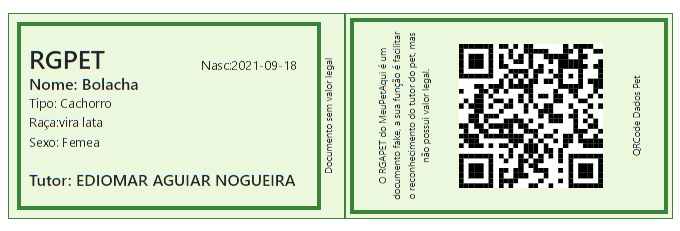
\includegraphics[width=15cm]{arquivos/Figuras/image18.png}
     \caption{RGA}
         \label{fig:RGA}
\end{figure}

\newpage
\subsection{Cartão de Vacinas}
O cartão de vacinas consiste em uma subsessão do perfil do pet, onde os usuários podem cadastrar as vacinas e medicamentos administrados ao seu animal de estimação. Essa funcionalidade proporciona um maior controle das medicações e datas, permitindo que o usuário tenha um histórico completo e atualizado do tratamento do seu pet.

Além disso, o sistema oferece a possibilidade de fazer o download de um arquivo de imagem contendo a listagem das medicações registradas. Essa funcionalidade é especialmente útil quando é necessário compartilhar as informações com um veterinário ou em situações de emergência. Com o arquivo em mãos, o usuário pode apresentar de forma clara e concisa os medicamentos administrados ao seu pet, facilitando o diagnóstico e tratamento veterinário. (Figura \ref{fig:CartaoDeVacinas}).
\begin{figure}[htb]
     \centering
     \FonteFig{Elaborado pelo autor}
     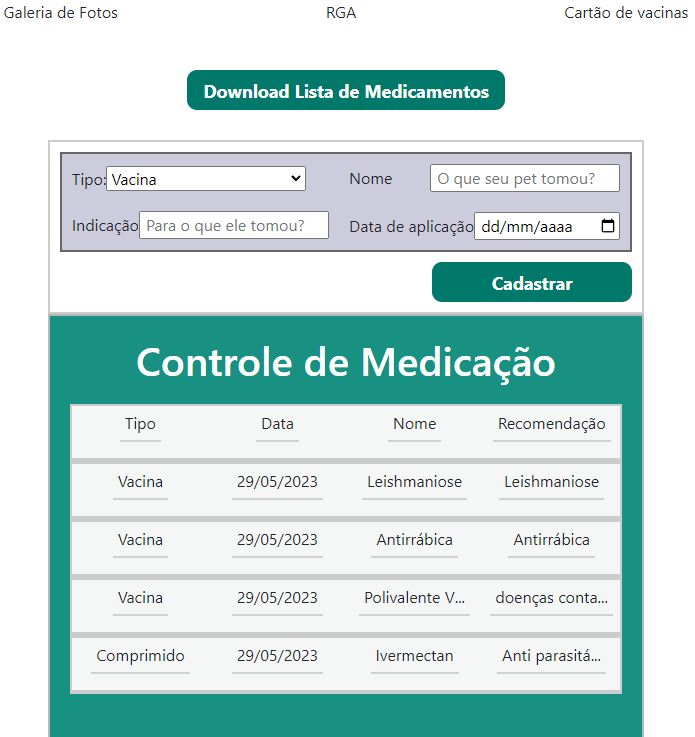
\includegraphics[width=12cm]{arquivos/Figuras/cartaovacinas.png}
     \caption{Cartão de Vacinas}
         \label{fig:CartaoDeVacinas}
\end{figure}

\begin{table}[htbp]
\centering
\renewcommand{\arraystretch}{1.5}
\begin{tabular}{|c|>{\centering\arraybackslash}m{6cm}|c|}
\hline
\textbf{Link} & \textbf{QR Code} \\
\hline
\href{https://drive.google.com/file/d/1vI_Te1o12bq-3kZFpDAnJCw6DOH5CZHc/view?usp=drive_link}{Armazenamento em Google Drive} & 
\includegraphics[width=3.5cm]{arquivos/ImgLinks/funcionalidadesPet.png} \\
\hline
\end{tabular}
\caption*{Vídeo sobre funcionalidades do perfil do pet - Fonte: Próprio autor}
\end{table}

\newpage
\section{Gerar Alertas}
Ao entrar na página do perfil do pet na plataforma, o usuário tem a opção de gerar alertas através de um botão específico. Ao clicar no botão, é redirecionado para uma página de criação de alertas, onde pode preencher um formulário com informações relevantes para a resolução da situação cadastrada. Esse formulário permite cadastrar situações como a perda ou o encontro de um animal, a divulgação de um pet para adoção ou quando se tratar de uma ONG, a busca por apoio financeiro para custeio de cuidados veterinários.

O formulário de criação de alertas solicita a foto mais recente do pet em questão, a descrição da situação, a situação em que se encontra (perdido, encontrado, para adoção ou necessitando de tratamento), data da ocorrência, telefone para contato do responsável pelo alerta e localização de referência da ocorrência. O local inicial é fornecido por meio do cadastro do usuário, mas é possível atualizá-lo durante o preenchimento do formulário de alerta, por exemplo, se o pet se perdeu durante um passeio em um local diferente do seu endereço cadastrado. (Figura \ref{fig:GerarAlertas}).
\newpage

\begin{figure}[htb]
     \centering
     \FonteFig{Elaborado pelo autor}
     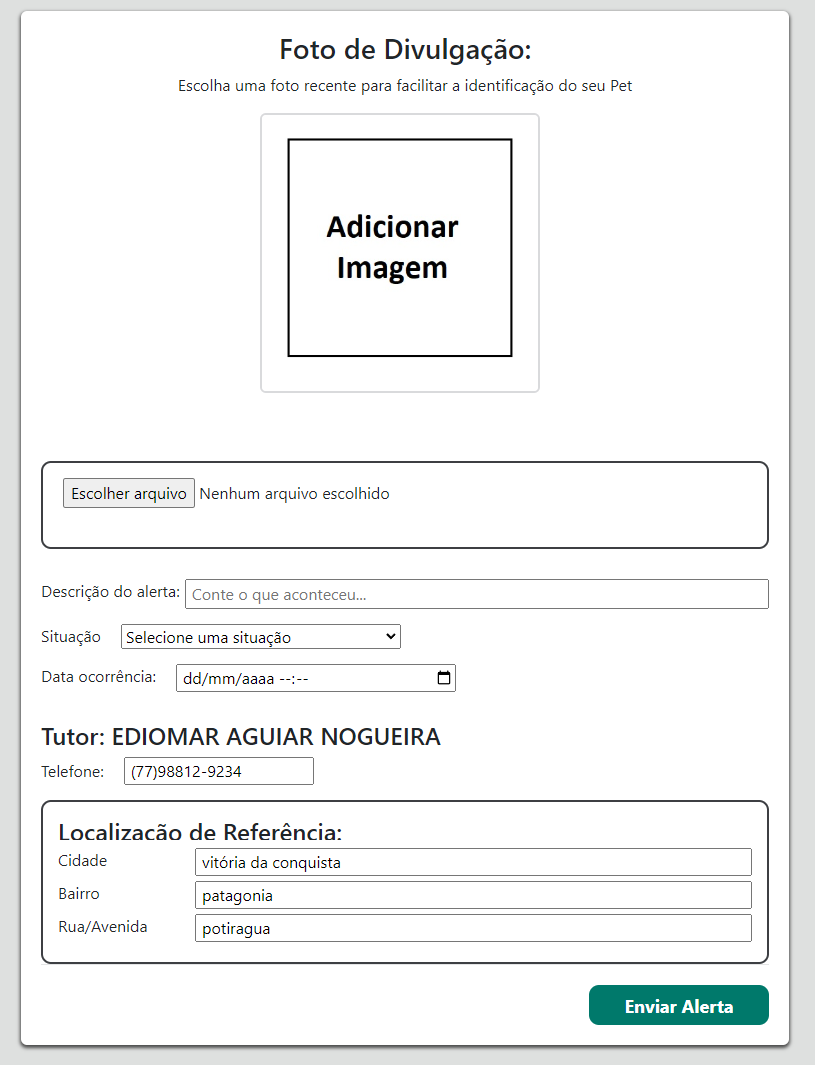
\includegraphics[width=12cm]{arquivos/Figuras/image1.png}
     \caption{Formulário de Geraração de Alertas}
         \label{fig:GerarAlertas}
\end{figure}

\begin{table}[htbp]
\centering
\renewcommand{\arraystretch}{1.5}
\begin{tabular}{|c|>{\centering\arraybackslash}m{6cm}|c|}
\hline
\textbf{Link} & \textbf{QR Code} \\
\hline
\href{https://drive.google.com/file/d/1s08Vz-h8y9M3bp_4HEkIN2xDcSTKl-AS/view?usp=drive_link}{Armazenamento em Google Drive} & 
\includegraphics[width=3.5cm]{arquivos/ImgLinks/formularioAlerta.png} \\
\hline
\end{tabular}
\caption*{Vídeo sobre envio de alerta - Fonte: Próprio autor}
\end{table}

\newpage
\subsection{Feed de Alertas}
O Feed de alertas segue a mesma lógica do Feed de posts, explicado na seção \ref{subsec:FeedPosts}. Assim, ele é formado por posts de divulgação gerados pelos usuários, a partir das informações inseridas no formulário de criação de alertas. Esses posts são adicionados ao feed de todos os amigos e seguidores do autor do alerta, ou aos usuários que estão dentro do raio de alcance da postagem, que por padrão é de 5 km.

Ao visualizar o feed, o usuário pode facilmente identificar qual a situação exposta por meio do título padronizado de acordo com a categoria do alerta. Para cães perdidos, o título é "Cão perdido! Você viu este doguinho por aí?"; para cães encontrados, "Cão encontrado! Ei, você conhece o dono deste cachorro?"; para cães disponíveis para adoção, "Cão para adoção! Tenha este doguinho como seu novo amigo..."; e para cães que precisam de tratamento veterinário, "Cão precisando de ajuda! Esse doguinho precisa de sua ajuda!". 	Para alertas gerados para gatos, as frases são idênticas, com a única diferença nas palavras que identificam a espécie do animal. Além disso, os posts são identificados por cores de acordo com seu tema: vermelho para animais perdidos, verde para animais encontrados, amarelo para animais disponíveis para adoção e preto para animais em tratamento.

Por fim, os alertas podem ser filtrados de acordo com suas categorias, facilitando a busca por determinados animais ou ocorrências.(Figura \ref{fig:FeedDeAlertas}).
\newpage

\begin{figure}[htb]
     \centering
     \FonteFig{Elaborado pelo autor}
     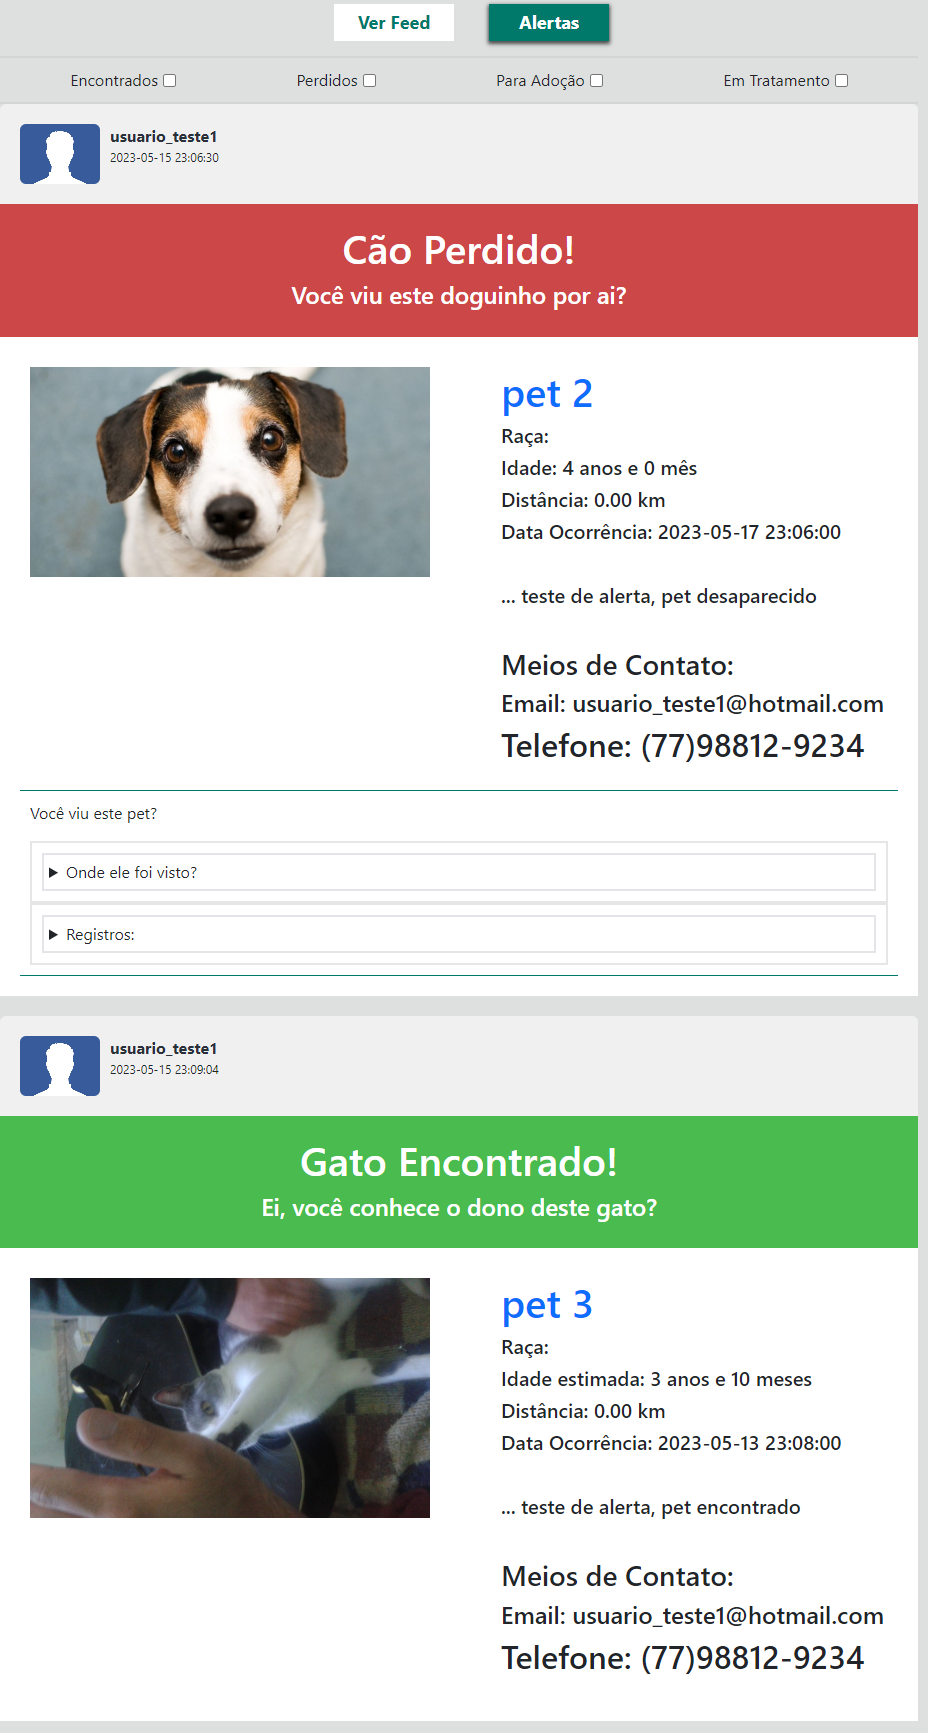
\includegraphics[width=9cm]{arquivos/Figuras/image19.png}
     \caption{Feed de Alertas}
         \label{fig:FeedDeAlertas}
\end{figure}

\newpage

\section{Rastreamento de Pets}

Os alertas de pets perdidos são uma ferramenta importante para ajudar a reunir animais com seus tutores. Além de fornecer os dados do tutor para contato, o formulário do alerta permite que outras pessoas que tenham visto o animal desaparecido ou um animal semelhante informem a localização em que ele foi avistado. O formulário de alerta para pet desaparecido solicita as seguintes informações: um comentário sobre o animal avistado, a data em que ele foi visto, a localização detalhada com cidade, bairro e rua, e caso disponível, a foto do animal para facilitar a identificação. Esses dados são fundamentais para ajudar na busca e recuperação dos pets desaparecidos. 
(Figura \ref{fig:FormularioRastreamento}).
\begin{figure}[htb]
     \centering
     \FonteFig{Elaborado pelo autor}
     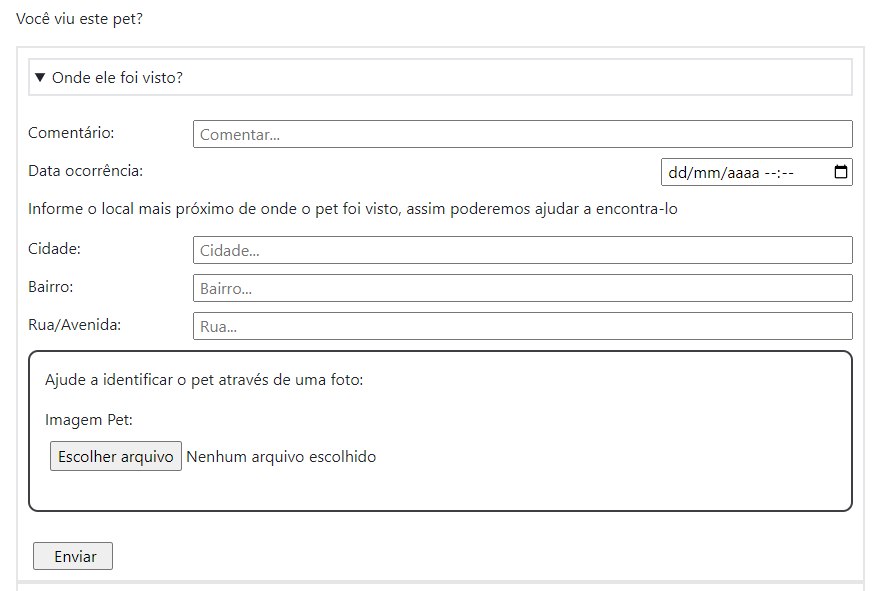
\includegraphics[width=14cm]{arquivos/Figuras/image3.png}
     \caption{Formulário de Rastreamento}
         \label{fig:FormularioRastreamento}
\end{figure}

\newpage
Ao coletar as informações de cidade, bairro e rua fornecidas pelos usuários que contribuem para a localização do pet perdido, a plataforma é capaz de reunir todas essas informações e gerar um mapa com os pontos em que o animal foi avistado. Além disso, as informações cadastradas pelos usuários, como comentários sobre o pet e a data em que foi visto, juntamente com a imagem anexada (se disponíveis), são exibidas na plataforma. Dessa forma, a ferramenta se torna uma participante ativa na busca pelo animal desaparecido, ajudando a reunir informações úteis e relevantes para a sua localização. (Figura \ref{fig:MapaRastreamento}).


\begin{figure}[htb]
     \centering
     \FonteFig{Elaborado pelo autor}
     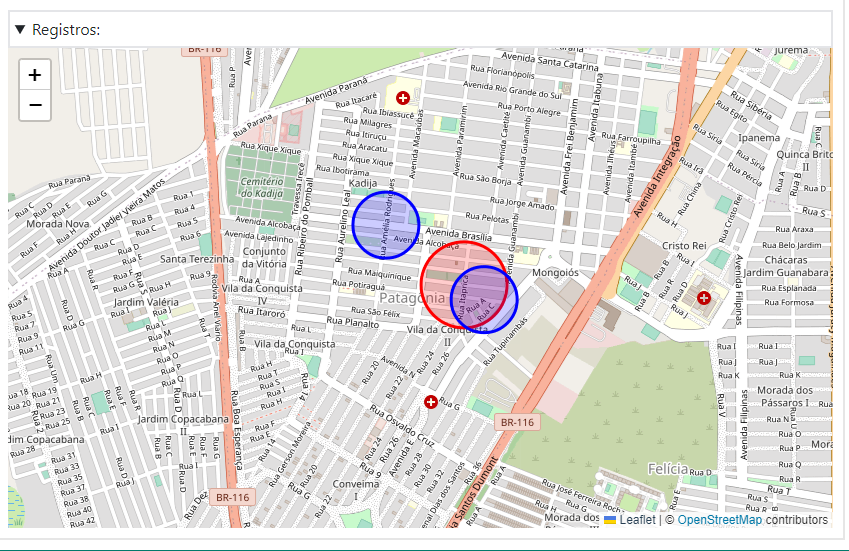
\includegraphics[width=14cm]{arquivos/Figuras/image10.png}
     \caption{Mapa de Rastreamento}
         \label{fig:MapaRastreamento}
\end{figure}

\begin{table}[htbp]
\centering
\renewcommand{\arraystretch}{1.5}
\begin{tabular}{|c|>{\centering\arraybackslash}m{6cm}|c|}
\hline
\textbf{Link} & \textbf{QR Code} \\
\hline
\href{https://drive.google.com/file/d/1WKvfjzqN_9fP20qKuA3kI_nFvi4fcJis/view?usp=drive_link}{Armazenamento em Google Drive} & 
\includegraphics[width=3.5cm]{arquivos/ImgLinks/alertas.png} \\
\hline
\end{tabular}
\caption*{Vídeo sobre alertas - Fonte: Próprio autor}
\end{table}

\newpage
\section{Pets de Ongs}

Os pets cadastrados por perfis de ONGs recebem destaque na plataforma, sendo facilmente acessados por meio do menu localizado na lateral direita, presente em todas as páginas. No menu de Pets de ONGs, os usuários têm acesso a páginas especializadas, organizadas de acordo com a nomenclatura correspondente. (Figura \ref{fig:PostOng}).

\begin{figure}[htb]
     \centering
     \FonteFig{Elaborado pelo autor}
     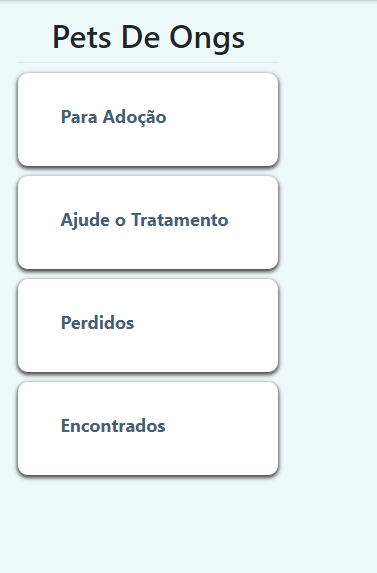
\includegraphics[width=6cm]{arquivos/Figuras/postong.png}
     \caption{Posts de ONGs}
         \label{fig:PostOng}
\end{figure}

As páginas dedicadas aos pets cadastrados pelas ONGs funcionam como um catálogo de animais, organizados por categorias específicas. Essas páginas exibem cards com informações básicas dos pets, como o nome da ONG responsável e a nomenclatura atribuída para identificar cada cão ou gato.

Ao clicar no nome da ONG, o usuário é redirecionado para a página de perfil da própria ONG, onde pode obter mais informações sobre a organização. Da mesma forma, ao clicar no nome ou na imagem do pet, o usuário é direcionado para o perfil individual do animal. No perfil do pet, é possível ter acesso a informações mais detalhadas e relevantes sobre o animal em questão. (Figura \ref{fig:petsDeOngs}).
\begin{figure}[htb]
     \centering
     \FonteFig{Elaborado pelo autor}
     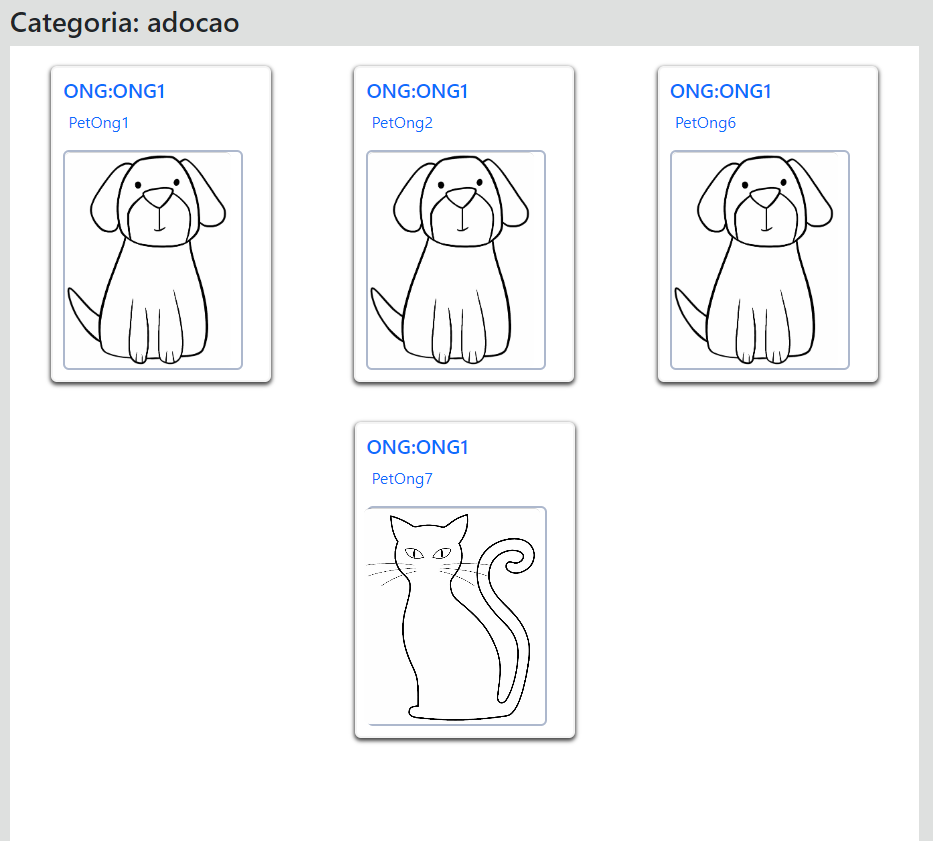
\includegraphics[width=14cm]{arquivos/Figuras/petscategoriaadocao.png}
     \caption{Pets Para Adoção Cadastrados Por ONG}
         \label{fig:petsDeOngs}
\end{figure}

\begin{table}[htbp]
\centering
\renewcommand{\arraystretch}{1.5}
\begin{tabular}{|c|>{\centering\arraybackslash}m{6cm}|c|}
\hline
\textbf{Link} & \textbf{QR Code} \\
\hline
\href{https://drive.google.com/file/d/1dkYJRDHbpXpmBwEDp8kkl79o4_4MUrHC/view?usp=drive_link}{Armazenamento em Google Drive} & 
\includegraphics[width=3.5cm]{arquivos/ImgLinks/PetsPorOngs.png} \\
\hline
\end{tabular}
\caption*{Vídeo sobre pets cadastrados por ongs - Fonte: Próprio autor}
\end{table}

\newpage
\chapter{Modelagem}
\section{Requisitos Funcionais}
Os requisitos funcionais são declarações que descrevem as funções que o sistema deve oferecer, incluindo sua resposta a entradas específicas e o comportamento esperado em diferentes situações \cite[p,83]{Sommerville}. Nesta subSeção, apresentam-se os requisitos funcionais (RF) do sistema, juntamente com detalhes sobre suas complexidades e prioridades. A fim de estabelecer a ordem de importância desses requisitos, foram adotadas as classificações "essencial", "importante" e "desejável".
\begin{itemize}[leftmargin=2cm]
\item[RF01 -] {\bf Cadastro de Usuário:} O sistema deve ser capaz de cadastrar usuários. O cadastro deve ser realizado com as seguintes informações: nome, e-mail, senha (obedecendo critérios de força definidos), confirmação de senha, categoria de usuário (usuário ou ONG), número de telefone e data de nascimento. Antes de finalizar o cadastro, o sistema deve realizar validações para verificar se todos os campos obrigatórios foram preenchidos corretamente, se a senha atende aos critérios predefinidos e se a confirmação de senha é idêntica à senha informada.
\item[RF02 -] {\bf Busca de Usuário:} O sistema deve permitir a busca por dados de usuário. Essa funcionalidade permitirá que o usuário edite seus próprios dados.
\item[RF03 -] {\bf Edição de Usuário:} A plataforma deve fornecer meios para que o usuário atualize seus dados cadastrados.
\item[RF04 -] {\bf Criação de Posts:} A plataforma deve permitir que o usuário crie posts e os publique em seu feed. Os posts podem conter texto, imagens e marcações de pets pertencentes ao usuário.
\item[RF05 -] {\bf Feed de Posts:} A plataforma deve organizar os posts em ordem decrescente, exibindo os mais recentes primeiro. O feed de posts deve apresentar apenas os posts criados pelo usuário e pelos usuários vinculados a ele.
\item[RF06 -] {\bf Interação com Posts:} O sistema deve permitir que os usuários interajam com os posts. Cada post deve permitir a adição de comentários e a marcação de "curtir".
\item[RF07 -] {\bf Vínculo Entre Usuários:}  O sistema deve oferecer aos usuários a possibilidade de seguir, ser seguido ou deixar de seguir outros usuários.
\item[RF08 -] {\bf Perfil de Usuário:} A plataforma deve disponibilizar aos usuários um perfil exclusivo, onde serão exibidos os dados cadastrados por eles. Esse perfil permitirá a visualização e a edição rápida das informações fornecidas durante o cadastro. O usuário poderá visualizar e atualizar dados como nome, foto, informações de contato, preferências e outras informações relevantes.
\item[RF09 -] {\bf Galeria de Fotos:} A plataforma deve coletar e armazenar as imagens postadas pelos usuários. Quando uma imagem estiver marcada com um pet, ela será exibida tanto no perfil do usuário quanto no perfil do pet marcado. Caso a imagem não possua marcação de pet, ela será exibida apenas no perfil do usuário.
\item[RF10 -] {\bf Cadastro de Pet:} A plataforma deve permitir o cadastro de pets. O cadastro deve incluir informações como nome, espécie, data de nascimento e situação do pet. A situação do pet poderá ser uma das seguintes opções:
\begin{itemize}[leftmargin=2cm]
\item Meus pets: para pets que pertencem ao usuário.
\item Encontrei este pet: para pets encontrados pelo usuário.
\item Pet desaparecido: para pets que estão desaparecidos.
\item Pet em tratamento (disponível apenas para perfis de usuário do tipo ONG): para pets que estão sob cuidados de uma ONG e em processo de tratamento.
\end{itemize}
\item[RF11 -] {\bf Visualização dos Pets:} A plataforma deve proporcionar ao usuário a visualização dos seus pets, organizados de acordo com diferentes situações. Essas situações podem ser categorizadas da seguinte forma:
\begin{itemize}[leftmargin=2cm]
\item Meus pets: exibe os pets que pertencem ao usuário.
\item Encontrei este pet: exibe os pets que o usuário encontrou.
\item Pet desaparecido: exibe os pets que estão desaparecidos.
\item Pet em tratamento (disponível apenas para perfis de usuário do tipo ONG): exibe os pets que estão sob cuidados da ONG e em tratamento.
\end{itemize}
\item[RF12 -] {\bf Perfil do Pet:} A plataforma deve disponibilizar perfis exclusivos para cada um dos pets cadastrados pelo usuário. Esses perfis devem exibir as informações cadastrais do pet, como nome, foto, porte, pelagem e outras informações relevantes. O usuário poderá visualizar e atualizar os dados cadastrais do pet por meio desse perfil.
\item[RF13 -] {\bf Busca de Pet:} O sistema deve permitir a busca por dados do pet. Essa funcionalidade servirá para que o usuário possa editar os dados do seu pet.
\item[RF14 -] {\bf Edição de Pet:} A plataforma deve fornecer meios para que o usuário possa atualizar os dados do seu pet.
\item[RF15 -] {\bf Registro Geral de Animal (RGA):} A plataforma deve atribuir a cada pet um Registro Geral de Animal (RGA) exclusivo. O RGA conterá informações importantes sobre o pet, como nome, tipo (cão, gato), raça, sexo, data de nascimento e nome do tutor. Além dos dados cadastrais, o RGA do pet incluirá um QR code exclusivo que fornecerá acesso direto ao perfil do pet na plataforma.
\item[RF16 -] {\bf Cartão de Vacinas:} A plataforma deve permitir o cadastro e visualização das medicações e vacinas aplicadas ao pet. Isso permitirá o registro e acompanhamento das intervenções medicamentosas e imunizações realizadas ao longo do tempo.
\item[RF17 -] {\bf Gerar Alertas:} O sistema deve permitir ao usuário a criação de alertas. O usuário deve fornecer informaçãoes: Foto recente do pet, descrição da situação, a situação em que se encontra (perdido, encontrado, para adoção ou necessitando de tratamento), data da ocorrência.
\item[RF18 -] {\bf Feed de Alertas:} A plafataforma deve organizar os alertas em ordem decrescente,  exibindo os mais recentes primeiro. O feed de alertas deve apresentar os alertas gerados pelo próprio usuário e por todos os demais usuários da plataforma.
\item[RF19 -] {\bf Rastreamento:} O sistema deve ser capaz de registrar a localização dos usuários e de seus pets. 
\item[RF20 -] {\bf Rastreamento de Pets:} Em alertas de pets desaparecidos a plataforma deve permitir que os usuários informem quando virem o pet, fornecendo informações: Comentário, data em que foi visto, cidade, bairro, rua/avenida e imagem.
\item[RF21 -] {\bf Mapeamento :} A plataforma deve oferecer um recurso de mapeamento para exibir o histórico de registro de avistamento de um pet desaparecido.
\item[RF22 -] {\bf Agrupamento de Pets por ONGs:} A plataforma deve disponibilizar páginas específicas para cada situação de cadastro de pets realizados por ONGs. As situações de cadastro podem incluir:
\begin{itemize}[leftmargin=2cm]
\item Pets para adoção: Nessa página, serão exibidos os pets cadastrados pelas ONGs que estão disponíveis para adoção. O usuário devem visualizar informações sobre cada pet, como nome, espécie, raça, idade e características, além de entrar em contato com a respectiva ONG responsável pela adoção.
\item Pets em tratamento: Nessa página, serão listados os pets que estão em tratamento pelas ONGs. O usuário deve verificar quais animais estão recebendo cuidados veterinários, quais tratamentos estão sendo realizados e acompanhar o progresso de recuperação de cada pet.
\item Pets perdidos: Nessa página, serão exibidos os pets cadastrados pelas ONGs que estão desaparecidos. O usuário deve visualizar informações sobre cada pet perdido, como nome, espécie, raça, características e a data em que desapareceu.
\newpage
\item Pets encontrados: Nessa página, serão exibidos os pets que foram encontrados pelas ONGs e estão aguardando a identificação de seus tutores. O usuário deve verificar as informações dos pets, como local e data do encontro, características e entrar em contato com a ONG responsável para reivindicar o pet perdido.

\end{itemize}
O meio de exibição dos pets deve permitir fácil acesso para as páginas de perfil dos pets.

\end{itemize}


\begin{table}[htb]
    \centering
    \caption{Grau de complexidade e prioridade dos requisitos funcinoais.}
    \begin{tabular}{|l|c|c|}
        \hline
        \textbf{Requisito Funcional} & \textbf{Complexidade} & \textbf{Prioridade}\\
        \hline
        RF01 & Baixa & Essensial\\
        \hline
        RF02 & Baixa & Importante\\
        \hline
        RF03 & Baixa & Desejável\\
        \hline
        RF04 & Alta & Importante\\
        \hline
        RF05 & Média & Importante\\
        \hline
        RF06 & Média & Desejável\\
        \hline
        RF07 & Alta & Desejável\\
        \hline
        RF08 & Média & Importante\\
        \hline
        RF09 & Baixa & Desejável\\
        \hline
        RF10 & Baixa & Essensial\\
        \hline
        RF11 & Baixa & Essensial\\
        \hline
        RF12 & Média & Importante\\
        \hline
        RF13 & Baixa & Importante\\
        \hline
        RF14 & Baixa & Desejável\\
        \hline
        RF15 & Baixa & Desejável\\
        \hline
        RF16 & Média & Desejável\\
        \hline
        RF17 & Alta & Importante\\
        \hline
        RF18 & Média & Importante\\
        \hline
        RF19 & Baixa & Essensial\\
        \hline
        RF20 & Média & Essensial\\
        \hline
        RF21 & Alta & Essensial\\
        \hline
        RF22 & Média & Essensial\\
        \hline
        \hline
    \end{tabular}    
    \caption*{\small Fonte: Elaborado pelo autor}
    \label{tab:Plataformas2}
\end{table}

\newpage
\section{Requisitos Não-Funcionais}
Os requisitos não-funcionais, de acordo com \citeonline[p.83]{Sommerville}, "são restrições sobre os serviços ou as funções oferecidos pelo sistema". Nesta subseção, serão apresentados os requisitos que impõem restrições à utilização do sistema e ao seu desenvolvimento, levando em consideração critérios e restrições que afetam sua operação e desempenho.

\begin{itemize}[leftmargin=2cm]
  \item[RN01 -] O MeuPetAqui deve utilizar \gls{API} (Interface de Programação de Aplicação)  de geolocalização Open Source por garantir a liberdade de adaptar e modificar o sistema de acordo com os requisitos específicos, além de proporcionar uma solução economicamente viável e sustentável.
  \item[RN02 -] A plataforma deve utilizar um Banco de Dados Open Source pela disponibilidade do código-fonte, permitir maior flexibilidade e customização, além de ser uma opção econômica e vantagens oferecidas pela comunidade de desenvolvedores.
  \item[RN03 -] O layout da plataforma deve ser projetado levando em consideração os padrões de disposição de elementos encontrados em outras redes sociais populares. O usuário deve ter uma experiência familiar e intuitiva ao acessar o sistema.
  \item[RN04 -] A navegação entra as páginas deve ser rápida e fluida.
  \item[RN05 -] Alertas devem possuir titulo e cores distintas para cada variação de situação de alerta.
\end{itemize}

\newpage

\section{Casos de Uso}
Os casos de uso desempenham um papel fundamental na engenharia de requisitos de um sistema. Eles são representações textuais das funcionalidades do sistema, descrevendo como os atores (usuários ou outros sistemas) interagem com o sistema em diferentes situações. Os casos de uso fornecem uma visão sucinta e organizada de como o sistema deve funcionar, facilitando o entendimento dos requisitos e o trabalho da equipe de desenvolvimento \cite{Guedes}.

Nesta seção, será explorado o diagrama de casos de uso da plataforma MeuPetAqui. (Figura \ref{fig:casosDeUso}).
\begin{figure}[htb]
     \centering
     \FonteFig{Elaborado pelo autor}
     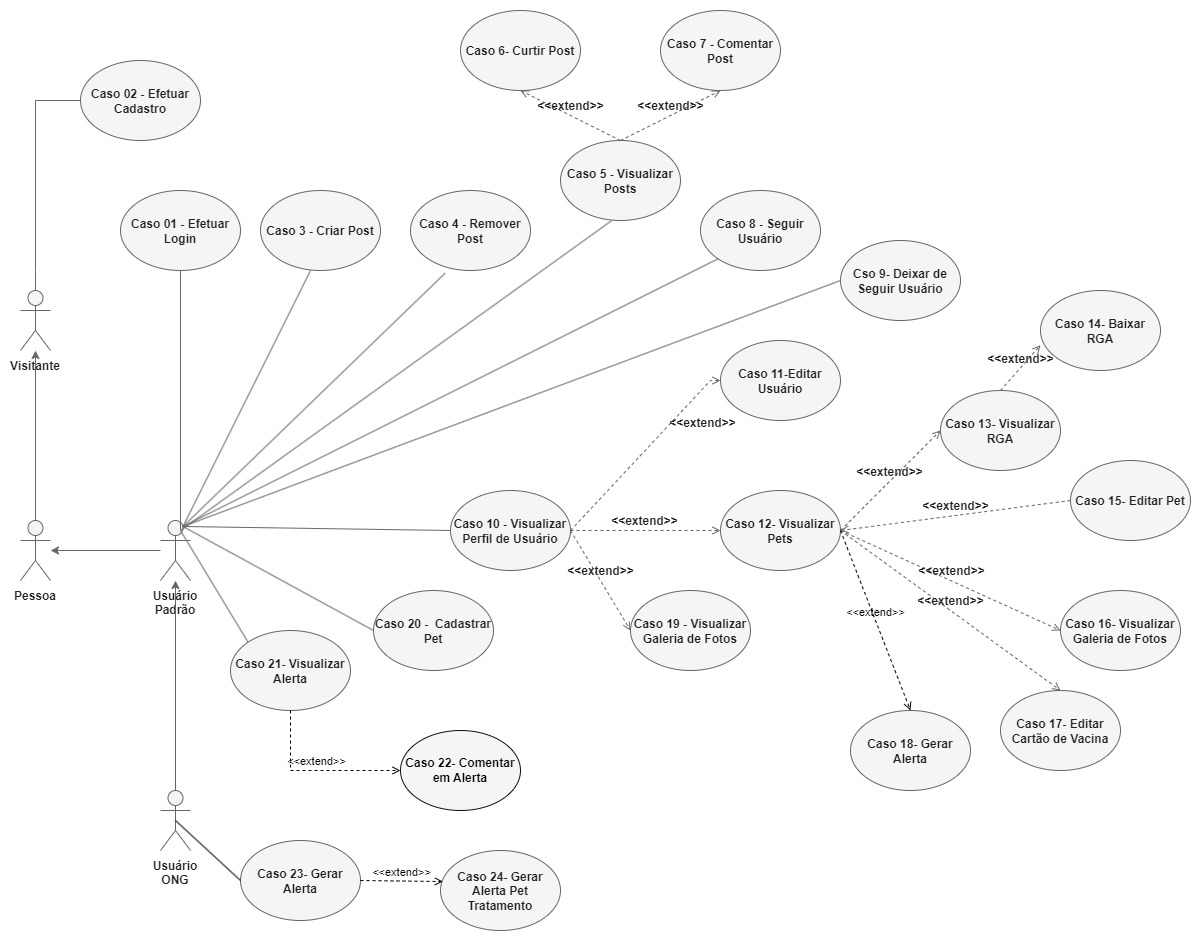
\includegraphics[width=15cm]{arquivos/Figuras/diagrama.jpg}
     \caption{Diagrama casos de uso}
         \label{fig:casosDeUso}
\end{figure}

\newpage
Na Tabela \ref{tab:tabela6.2}, é exposto um resumo dos fluxos básicos e alternativos do MeuPetAqui.

\begin{longtable}{|p{4cm}|p{9cm}|}
\caption{Resumo dos fluxos básicos do MeuPetAqui.}
\label{tab:tabela6.2} \\
\hline
\textbf{Caso de Uso} & \textbf{Descrição} \\
\hline
\endfirsthead

\caption*{\small Continuação da tabela \ref{tab:tabela6.2}} \\
\hline
\textbf{Caso de Uso} & \textbf{Descrição} \\
\hline
\endhead
    \hline
    CASO 01 - Efetuar Login & O usuário preenche os campos de e-mail e senha na tela de login e clica em "Entrar". O sistema valida os dados e realiza o login. \\
    \hline
    CASO 02 - Efetuar Cadastro & O usuário clica em "Efetuar Cadastro", preenche os campos do formulário e clica em "Registrar-se". O sistema avalia se todos os campos obrigatórios foram preenchidos corretamente e efetiva o cadastro.\\
    \hline
    CASO 03 - Criar Post & O usuário decide criar um post na tela inicial da plataforma. Ele pode preencher a área de texto, fazer upload de uma imagem e marcar seus pets na postagem. Após configurar o post, o usuário clica em "Enviar". O sistema valida a imagem e realiza a postagem.\\
    \hline
    CASO 04 - Remover Post & O usuário pode remover um post clicando no ícone de lixeira presente no post, desde que o post seja de sua autoria. O sistema exclui a postagem do feed.\\
    \hline
    CASO 05 - Visualizar Posts & O usuário clica em "Feed" na tela inicial para visualizar os posts. Ao rolar até o final do feed, ele pode carregar mais postagens clicando em "Ver mais". O sistema exibe inicialmente 6 posts e adiciona mais 6 a cada solicitação de "Ver mais".\\
    \hline
    CASO 06 - Curtir Post & O usuário pode curtir um post clicando no ícone de uma pata presente em cada post. A plataforma incrementa o contador de curtidas do post.\\
    \hline
    CASO 07 - Comentar Post & O usuário preenche o campo de comentário localizado abaixo do post e clica em "Enviar". A plataforma realiza o envio do comentário.\\
    \hline
    CASO 08 - Seguir Usuário & O usuário navega pela lista de usuários em "Próximos de você" na tela inicial e clica em "Seguir" para seguir um usuário. A plataforma realiza a ação de seguir o usuário.\\
    \hline
    CASO 09 - Deixar de Seguir Usuário & O usuário acessa sua guia "Meu perfil" na tela inicial, em seguida, na página de perfil, clica em "Seguindo" e navega até o usuário que deseja deixar de seguir. Caso o usuário não esteja inicialmente na lista, o usuário pode carregar mais usuários seguidos clicando em "Ver mais". Após encontrar o usuário desejado para deixar de seguir, o usuário clica em "Não seguir" e a plataforma remove o usuário da lista de seguidos.\\
    \hline
    CASO 10 - Visualizar Perfil de Usuário & O usuário pode acessar o perfil de um usuário clicando no nome dele nos posts, na lista de "Próximos de você" e nas relações de "Amigos", "Seguidores" e "Seguindo". Para acessar seu próprio perfil, o usuário clica em "Meu perfil" ou em sua própria identificação nos posts. A plataforma carrega a página correspondente ao usuário.\\
    \hline
    CASO 11 - Editar Usuário & O usuário acessa seu perfil de usuário e clica em "Configurar" para editar o perfil. Ele pode alterar os dados e arquivos e finalizar a edição clicando em "Atualizar Dados". A plataforma substitui os dados e arquivos antigos pelos novos. \\
    \hline
    CASO 12 - Visualizar Pets & O usuário clica em "Pets" na página inicial ou em um perfil de usuário para visualizar os pets. A plataforma carrega a página de exibição dos pets.\\
    \hline
    CASO 13 - Visualizar RGA & O usuário clica no card de perfil de um pet e caso o pet seja cadastrado por ele, a opção "RGA" estará disponível. O usuário clica em "RGA" e a plataforma exibe o RGA.\\
    \hline
    CASO 14 - Baixar RGA & O usuário acessa o perfil de um pet cadastrado por ele, clica em "RGA" e, na exibição do RGA, clica em "Download RGA Fake". A plataforma faz o download da imagem do RGA para a máquina do usuário.\\
    \hline
    CASO 15 - Editar Pet & O usuário acessa a página de perfil de um pet cadastrado por ele e clica em "Configurar" para editar o pet. Ele pode alterar os dados e arquivos e finalizar a edição clicando em "Atualizar Dados". A plataforma substitui os dados e arquivos antigos pelos novos.\\
    \hline
    CASO 16 - Visualizar Galeria de Fotos do Usuário & O usuário clica em "Galeria de Fotos" na página inicial ou no perfil de um usuário para visualizar as fotos postadas. A plataforma carrega a página de exibição das imagens.\\
    \hline
    CASO 17 - Editar Cartão de Vacina & O usuário clica no card de perfil de um pet cadastrado por ele e, caso a opção "Cartão de Vacina" esteja disponível, preenche os campos informando as vacinas e medicamentos que o pet já recebeu e as respectivas datas. A plataforma atualiza os dados de medicação.\\
    \hline
    CASO 18 - Visualizar Galeria de Fotos do Pet & O usuário clica no card de perfil de um pet e, após acessar o perfil do pet, clica em "Galeria de Fotos". A plataforma exibe a galeria de fotos daquele pet.\\
    \hline
    CASO 19 - Cadastrar Pet & O usuário clica em "Pets" na página inicial. Na página de listagem dos pets do usuário, ele clica em "Novo Pet" e fornece os dados iniciais do pet (Nome, espécie, data de nascimento, situação). Ao clicar em "Cadastrar Pet", a plataforma realiza o cadastro do pet.\\
    \hline
    CASO 20 - Gerar Alerta & O usuário clica no card de perfil de um pet cadastrado por ele e, em seguida, clica em "Gerar Alerta". Ele informa a imagem do pet, a descrição da ocorrência, a situação correspondente, a data e hora, telefone de contato e localização de referência da ocorrência. A plataforma registra o alerta e o compartilha com os demais usuários do sistema próximos a um raio de 5 km e com os contatos do usuário.\\
    \hline
    CASO 21 - Visualizar Alerta & O usuário clica em "Ver Alertas" na tela inicial para visualizar os alertas. Ao rolar até o final do feed de alertas, ele pode carregar mais clicando em "Ver mais". O sistema exibe inicialmente 6 alertas e adiciona mais 6 a cada solicitação de "Ver mais".\\
    \hline
    CASO 22 - Comentar Alerta & O usuário, ao visualizar um alerta do tipo "Pet desaparecido", clica em "Onde ele foi visto" para informar que viu o pet. Ele preenche as informações do comentário, data em que viu o pet, cidade, bairro e rua onde o pet foi visto. O usuário pode carregar uma imagem do pet encontrado e, em seguida, clica em "Enviar". A plataforma cadastra o registro.\\
    \hline
    CASO 23 - Gerar Alerta - ONG & O usuário clica no card de perfil de um pet cadastrado por ele e, em seguida, clica em "Gerar Alerta". Ele informa a imagem do pet, a descrição da ocorrência, a situação correspondente, a data e hora, telefone de contato e localização de referência da ocorrência. A plataforma registra o alerta e o compartilha com os demais usuários do sistema.\\
    \hline
    CASO 24 - Gerar Alerta - ONG (Em Tratamento) & O usuário da categoria ONG clica no card de perfil de um pet cadastrado por ele e, em seguida, clica em "Gerar Alerta". Ele informa a imagem do pet, a descrição da ocorrência, a situação correspondente (além das opções padrão, a opção "Pet em tratamento" está disponível), a data e hora, telefone de contato e localização de referência da ocorrência. A plataforma registra o alerta e o compartilha com os demais usuários do sistema.\\
    \hline
\end{longtable}

\newpage
\section{Arquitetura}

Neste seção, serão apresentados os detalhes da arquitetura utilizada na construção do MeuPetAqui, uma rede social dedicada aos donos de pets, ONGs e protetores de animais em Vitória da Conquista. O principal objetivo desta seção é fornecer uma visão abrangente dos componentes e tecnologias empregados, visando a criação de um sistema funcional, de alto desempenho, facilmente mantido e com capacidade de evolução.

A arquitetura do MeuPetAqui foi concebida levando em consideração a necessidade de criar uma plataforma que atendesse às demandas específicas dos usuários, bem como garantir a escalabilidade e a robustez do sistema. Para isso, foram definidos os componentes que serão descritos no decorrer deste segmento.
\subsection{Padrão Arquitetural}
O MeuPetAqui seguiu o padrão de arquitetura Model-View-Controller, podendo ser observado a divisão de cadamadas na construção do sistema.
\begin{itemize}
   \item A camada Model do MeuPetAqui abriga as classes responsáveis pelo controle lógico da plataforma, abrangendo as relações entre usuários, pets, posts, alertas e outros segmentos. Essa camada inclui as seguintes classes Models: AlertComment, Alerts, LocationPet, Pet, Post, PostComment, PostLike, RGA, User, UserRelation, UserRelationsPet e VaccineCard. Essas classes são responsáveis pela interação com o banco de dados, executando tarefas de leitura, gravação, atualização e exclusão de dados.
    \item A camada View é responsável por fornecer ao usuário a visualização e inserção de dados na plataforma. As páginas pertencentes à camada View recebem as informações dos Controllers e as apresentam ao usuário. Além disso, elas também recebem as entradas de dados dos usuários e as encaminham para o processamento pelos Controllers. A camada View desempenha um papel crucial na interação entre o usuário e a plataforma, garantindo uma experiência visualmente agradável e intuitiva. É por meio da camada View que os usuários podem interagir com os recursos e funcionalidades oferecidos pela aplicação.
    \item A camada Controller é responsável pela intermediação entre os Models e as Views, facilitando a troca de dados. Nessa camada, as ações de entrada do usuário são interpretadas e os dados são preparados para fornecer as respostas adequadas ao usuário ou para permitir que os Models executem suas operações. As classes de Controllers utilizadas na aplicação são: AlertController, AuthController, FeedController, LocationController, MedicamentPetController, OngController, PetController, PostController e UserController. Essas classes desempenham um papel fundamental na lógica da aplicação, coordenando as diferentes operações e garantindo a interação adequada entre os modelos de dados e as interfaces de usuário.
\end{itemize}
A plataforma estrutura-se em duas grantes partes, o FrontEnd e o Backend. No FrontEnd, foi utilizado o ReactJS para construção das Views, já o Backend consiste em uma API desenvolvida em Laravel. Essa estrutura segue a arquitetura MVC, em que o ReactJS é responsável pela camada de Views e o Laravel gerencia as camadas de Controllers e Models na API. 
\newpage
\subsection{Conhecendo mais do Backend}
\begin{itemize}
    \item {\bf Routes:} As Routes, ou rotas, desempenham um papel fundamental na arquitetura da API MeuPetAqui. Elas são responsáveis por conectar as extremidades (endpoints) da API e mapear as solicitações HTTP para as funções ou controladores específicos que as manipulam. No total, foram criadas 48 rotas para atender às diversas necessidades do sistema, abrangendo a criação e manipulação de perfis de usuário, perfis de pets, postagens e alertas. (Figura \ref{fig:Routes}).
    
    \begin{figure}[htb]
     \centering
     \FonteFig{Elaborado pelo autor}
     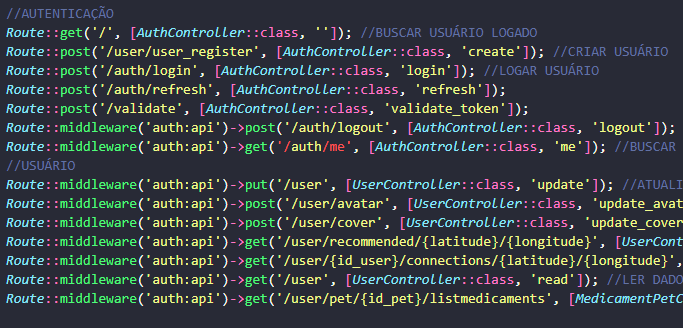
\includegraphics[width=14cm]{arquivos/Figuras/routes.png}
     \caption{Rotas MeuPetAqui}
         \label{fig:Routes}
\end{figure}
    \item {\bf Migrations:} As Migrations desempenham um papel essencial na atualização e gestão do banco de dados da aplicação. Elas fornecem uma abordagem estruturada para atualizar a estrutura do banco, permitindo o versionamento e garantindo a sincronia entre a estrutura atualmente em uso e a estrutura esperada pela plataforma. Isso é fundamental para manter a consistência entre o código da aplicação e o banco de dados, evitando problemas de incompatibilidade. Com as Migrations, é possível realizar alterações controladas e organizadas na estrutura do banco, como a criação ou modificação de tabelas, adição ou remoção de colunas e alteração de tipos de dados.
    \newpage
    \item {\bf JWT:} O \gls{JWT}\footnote{JWT (Json Web Token) é um padrão para autenticação e compartilhamento de informações. Baseado no formato JSON.} (JSON Web Token) foi implementado no MeuPetAqui para prover segurança na conexão do usuário ao sistema e no envio de requisições para a API. O seu funcionamento segue o seguinte fluxo:
    \begin{enumerate}
        \item Cliente solicita autenticação à API, informando email e senha.
        \item API autentica usuário e gera um JWT 
        \item Servidor envia o JWT para o usuário, este é armazenado em seu localstorage\footnote{ LocalStorage é uma propriedade que permite que sites e aplicativos JavaScript salvem pares chave-valor em um navegador da Web sem data de expiração.}.
        \item Nas demais solicitações o usuário envia o JWT junto à requisição, em seu cabeçalho.
        \item API verifica a autenticidade e integridade do JWT, se validado, processa a solicitação.
    \end{enumerate}
\end{itemize}
\newpage

\subsection{Conhecendo mais do FrontEnd}
\begin{itemize}
\item {\bf Axios:} No MeuPetAqui, o Axios foi escolhido como a biblioteca para realizar requisições HTTP à API devido à sua sintaxe amigável e fácil implementação. Ele proporcionou facilidade tanto para recuperar quanto enviar dados, além de lidar com o upload de arquivos. A capacidade de configurar cabeçalhos personalizados nas requisições e a assincronicidade das chamadas também foram motivos que contribuíram para a escolha do Axios. Essa integração permitiu uma comunicação eficiente entre o front-end e a API, proporcionando uma experiência de uso mais fluída para os usuários. (Figuras \ref{fig:componentes1}, \ref{fig:componentes2},\ref{fig:componentes3}).

\begin{figure}[htb]
     \centering
     \FonteFig{Elaborado pelo autor}
     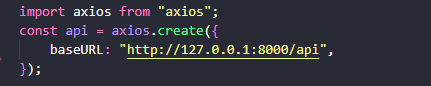
\includegraphics[width=12cm]{arquivos/Figuras/axios1.png}
     \caption{Configuração do Axios para requisições HTTP}
         \label{fig:componentes1}
\end{figure}
\begin{figure}[htb]
     \centering
     \FonteFig{Elaborado pelo autor}
     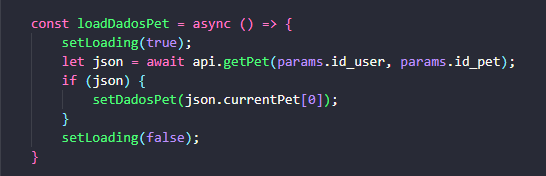
\includegraphics[width=12cm]{arquivos/Figuras/axios2.png}
     \caption{Uso da instância do axios para requisição Get}
         \label{fig:componentes2}
\end{figure}
\begin{figure}[htb]
     \centering
     \FonteFig{Elaborado pelo autor}
     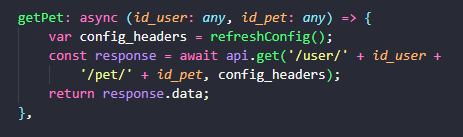
\includegraphics[width=12cm]{arquivos/Figuras/axios3.png}
     \caption{Uso da instância do axios para requisição Get}
         \label{fig:componentes3}
\end{figure}
\newpage
\item {\bf Componentização:} Ao aplicar o conceito de componentização, foi possivel manter o código organizado e claro, o que facilitou na aplicação de testes, manutenção e evolução da plataforma. Cada parte do sistema foi separada em componentes independentes e reutilizáveis, o que permitiu uma melhor divisão de responsabilidades e uma arquitetura mais modular. Isso possibilitou fazer alterações específicas em cada componente sem afetar o funcionamento global da plataforma. Além disso, a reutilização de componentes em diferentes partes do sistema trouxe uma maior eficiência no desenvolvimento e economia de tempo. 

A estrutura de separação em componentes foi implementada ao dividir os elementos comuns utilizados em várias páginas. Esses componentes foram elevados em níveis superiores na organização dos arquivos, o que facilitou sua atribuição quando necessário. Essa abordagem permitiu reutilizar os componentes em diferentes partes do sistema.(Figura \ref{fig:componentizacao}).

\begin{figure}[htb]
     \centering
     \FonteFig{Elaborado pelo autor}
     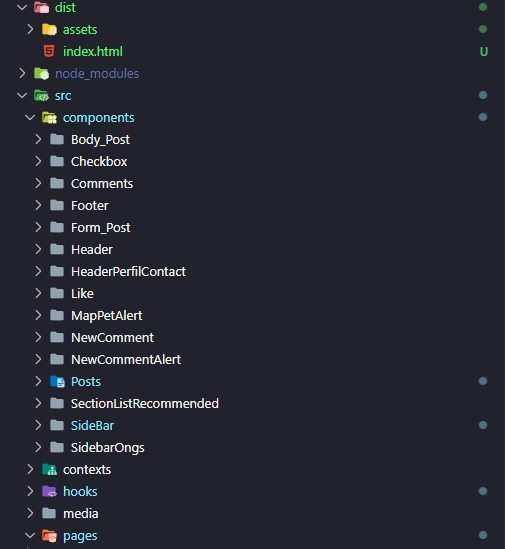
\includegraphics[width=10cm]{arquivos/Figuras/componentes1.png}
     \caption{Componentes de uso geral}
         \label{fig:componentizacao}
\end{figure}
\newpage
A segunda camada de separação em componentes foi implementada dentro das páginas, com o objetivo de reduzir a complexidade do código. Elementos individuais foram isolados e organizados em componentes específicos, que foram atribuídos às pastas correspondentes às respectivas páginas. Essa abordagem resultou em um código mais enxuto e claro para cada página, tornando a manutenção e compreensão do código mais fácil. (Figura \ref{fig:componentizacao2}).

\begin{figure}[htb]
     \centering
     \FonteFig{Elaborado pelo autor}
     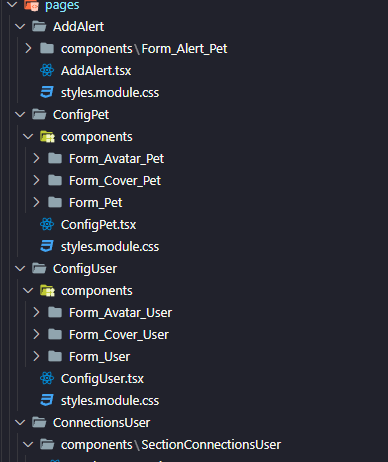
\includegraphics[width=8cm]{arquivos/Figuras/componentes2.png}
     \caption{Componentes de página}
         \label{fig:componentizacao2}
\end{figure}

\end{itemize}

\newpage
\subsection{API de Geolocalização - OpenStreetMap }
Para viabilizar a funcionalidade de rastreamento de pets perdidos, utilizou-se a API de Geolocalização da OpenStreetMap devido a algumas motivações específicas. Primeiramente, destaca-se a gratuidade do acesso a essa API. Além disso, a API da OpenStreetMap demonstrou ser de fácil utilização, o que agilizou o desenvolvimento do sistema.

Através do envio dos dados de localização, como cidade, bairro e rua, a API da OpenStreetMap é capaz de filtrar e retornar coordenadas aproximadas correspondentes ao local informado. (Figura \ref{fig:OpenStreetMap}). Essas coordenadas, representadas pela latitude e longitude, são então utilizadas pelo MeuPetAqui para processar a distância entre diferentes pontos geográficos. Essa funcionalidade é fundamental para o rastreamento dos pets perdidos, o mapeamento dos locais e também para direcionar alertas e recomendar usuários com base na proximidade geográfica.

Dessa forma, a integração com a API de Geolocalização da OpenStreetMap permite ao MeuPetAqui oferecer aos usuários recursos eficientes para a localização e rastreamento de seus animais de estimação perdidos.

\begin{figure}[htb]
     \centering
     \FonteFig{Elaborado pelo autor}
     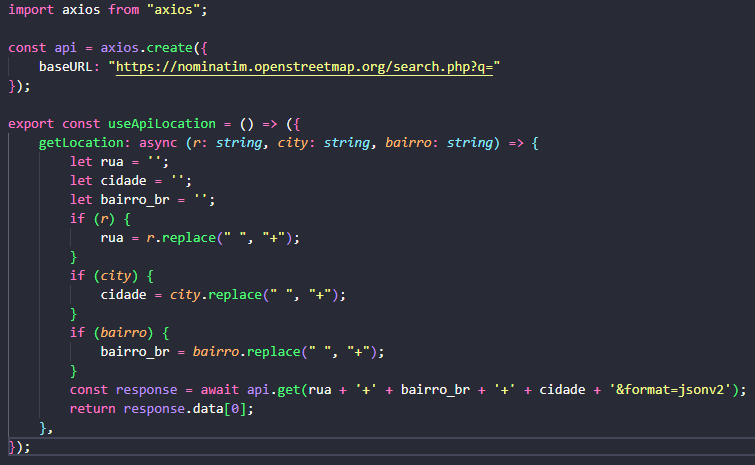
\includegraphics[width=14cm]{arquivos/Figuras/apigeolocalizacao.png}
     \caption{Integração com API OpenStreetMap}
         \label{fig:OpenStreetMap}
\end{figure}

\newpage
\section{Banco de Dados}

A implementação do banco de dados no MeuPetAqui teve como base o Sistema de Gerenciamento de Banco de Dados (SGBD) MariaDB\footnote{https://mariadb.org/}. Essa escolha foi motivada pela natureza Open Source do MariaDB, bem como pela existência de uma comunidade de desenvolvedores ativa, o que garante suporte e atualizações frequentes. Além disso, o MariaDB é conhecido por sua robustez e capacidade de escalabilidade, o que o torna adequado para atender às demandas de um sistema em crescimento como o MeuPetAqui.

No processo de diagramação do banco de dados, priorizou-se a perspectiva do usuário e dos pets como pontos centrais, desta forma a estrutura foi projetada para abranger as relações necessárias para prover as  funcionalidades e recursos previstos na plataforma. Dessa maneira, foram estabelecidas as conexões entre as diferentes entidades, levando em consideração as interações e dependências dos dados, resultando em um banco de dados bem organizado e adaptado às necessidades do MeuPetAqui. 

Em resumo, a escolha do MariaDB como SGBD e a diagramação centrada no usuário e nos pets foram aspectos fundamentais para garantir a eficiência, confiabilidade e escalabilidade do banco de dados do MeuPetAqui, contribuindo para o bom funcionamento e desenvolvimento contínuo da plataforma. Durante o desenvolvimento do MeuPetAqui, foi estabelecido como padrão a inclusão das entidades de status, data de registro e data de alteração de dados. Essa decisão foi tomada com o objetivo de possibilitar a expansão do sistema no futuro e garantir uma melhor gestão dos dados. A inclusão do status permite acompanhar o estado atual de cada registro, enquanto as datas de registro e alteração fornecem informações sobre quando os dados foram inseridos e atualizados. Esses campos adicionais contribuem para uma maior flexibilidade e escalabilidade do sistema, preparando-o para futuras melhorias e demandas crescentes de gerenciamento de dados.

\begin{itemize}
\item \textbf{Usuário:} armazena-se a categoria (identificando se o perfil é de usuário padrão ou de uma ONG), confirmação de ONG (validação do perfil), email, telefone, senha, nome, nome de conta do Instagram, nome de conta do Facebook, biografia, gênero, data de aniversário, latitude e longitude (para registro da localização de referência do usuário), profissão, cidade, bairro, rua em que o usuário mora, avatar e cover (para permitir personalização do perfil do usuário), status do usuário, data de registro e data de alteração de dados.

\item \textbf{Relações entre Usuários:} armazena-se o ID do usuário e o ID do usuário que é seguido por ele, o status desse registro, data de criação e data de possíveis alterações.

\item \textbf{Posts:} armazena-se o ID do usuário, a relação de pets marcados no post, o nome do arquivo da imagem inserida no post (se houver), a mensagem do post, status, data de registro e data de possíveis alterações.

\item \textbf{Comentários em Posts:} armazena-se o ID do post, o ID do usuário que efetua o comentário, o texto do comentário, status, data de registro e data de possíveis alterações.

\item \textbf{Likes em Posts:} armazena-se o ID do post, o ID do usuário que efetua a curtida, status, data de registro e data de possíveis alterações.

\item \textbf{Pet:} armazena-se o nome, ID do usuário que o registrou, espécie, raça, data de nascimento, biografia, status de castração, sexo, tamanho, comprimento da pelagem, situação em que o pet se encontra, avatar e cover (para personalização de perfil), status, data de cadastro e data de possíveis alterações.

\item \textbf{Registros de Vacinas:} armazena-se o ID do pet, o nome do medicamento ou vacina, status, data de criação e data de possíveis alterações.

\item \textbf{Alertas Gerados pelos Usuários:} armazena-se a foto do pet, ID do pet, ID do usuário responsável pelo cadastro do pet na plataforma, nome do tutor, descrição do alerta, situação ocorrida no alerta, cidade, bairro e rua, email e telefone para contato, latitude, longitude, status, data de cadastro e data de possíveis alterações.

\item \textbf{Comentários em Alertas:} armazena-se o ID do alerta, ID do usuário que comenta em um alerta, ID do pet, bairro, cidade e rua em que o pet foi avistado, imagem, comentário, data em que o pet foi avistado, latitude, longitude, status, data de registro e data de possíveis alterações.

\item \textbf{Registros de Rastreio de um Pet:} armazena-se o ID do pet, ID do post de alerta, ID dos comentários de localização, cidade, bairro, rua informados no comentário de rastreio, status, data de registro e data de possíveis alterações.
\end{itemize}

Essas entidades e seus respectivos atributos foram estabelecidos durante o desenvolvimento do MeuPetAqui, visando à integridade dos dados, à expansão futura do sistema e ao aprimoramento do gerenciamento das informações. Durante a construção do banco de dados do MeuPetAqui, adotou-se o padrão de nomenclatura em inglês para as entidades e atributos. Nas tabelas a seguir apresenta-se a relação de entidades e seus respectivos atributos:

\begin{table}[htb]
  \centering
  \caption{Relação de entidades e seus atributos tabela users}
  \begin{tabular}{|p{4cm}|}
    \hline
    \multicolumn{2}{|c|}{\textbf{Entidade} | \textbf{users}} \\
    \hline
    \multicolumn{1}{|c|}{\textbf{Atributos}} \\
    \hline
    id \\
    \hline
    category \\
    \hline
    confirmed\_ong \\
    email \\
    \hline
    phone \\
    \hline
    password \\
    \hline
    name \\
    \hline
    instagram \\
    \hline
    facebook \\
    \hline
    biography \\
    \hline
    genre \\
    \hline
    birthdate \\
    \hline
    latitude \\
    \hline
    longitude \\
    \hline
    work \\
    \hline
    road \\
    \hline
    city \\
    \hline
    district \\
    \hline
    avatar \\
    \hline
    cover \\
    \hline
    status \\
    \hline
    date\_register \\
    \hline
    date\_change \\
    \hline
   \hline
  \end{tabular}
  \caption*{\small Fonte: Elaborado pelo autor}
  \label{tab:Plataformas1}
\end{table}

\begin{table}[htb]
  \centering
  \caption{Relação de entidades e seus atributos tabela Pets}
  \begin{tabular}{|p{4cm}|}
    \hline
    \multicolumn{2}{|c|}{\textbf{Entidade} | \textbf{Pets}} \\
    \hline
    \multicolumn{1}{|c|}{\textbf{Atributos}} \\
    \hline
    id \\
    \hline
    name \\
    \hline
    id\_user \\
    \hline
    species \\
    \hline
    breed \\
    \hline
    biography \\
    \hline
    birthdate \\
    \hline
    castred \\
    \hline
    avatar \\
    \hline
    cover \\
    \hline
    genre \\
    \hline
    latitude \\
    \hline
    longitude \\
    \hline
    size \\
    \hline
    fur \\
    \hline
    situation \\
    \hline
    status \\
    \hline
    date\_register \\
    \hline
    date\_change \\
    \hline
  \end{tabular}
  \caption*{\small Fonte: Elaborado pelo autor}
  \label{tab:Plataformas1}
\end{table}

\begin{table}[htb]
  \centering
  \caption{Relação de entidades e seus atributos tabela users\_relations}
  \begin{tabular}{|p{4cm}|}
    \hline
    \multicolumn{2}{|c|}{\textbf{Entidade} | \textbf{user\_relations}} \\
    \hline
    \multicolumn{1}{|c|}{\textbf{Atributos}} \\
    \hline
    id \\
    \hline
    user\_from \\
    \hline
    user\_to \\
    \hline
    status \\
    \hline
    date\_register \\
    \hline
    date\_change \\
    \hline
  \end{tabular}
  \caption*{\small Fonte: Elaborado pelo autor}
  \label{tab:Plataformas1}
\end{table}

\begin{table}[htb]
  \centering
  \caption{Relação de entidades e seus atributos tabela posts}
  \begin{tabular}{|p{4cm}|}
    \hline
    \multicolumn{2}{|c|}{\textbf{Entidade} | \textbf{Posts}} \\
    \hline
    \multicolumn{1}{|c|}{\textbf{Atributos}} \\
    \hline
    id \\
    \hline
    situation \\
    \hline
    marked\_pets \\
    \hline
    type \\
    \hline
    body \\
    \hline
    subtitle\\
    \hline
    status \\
    \hline
    date\_register \\
    \hline
    date\_change \\
    \hline
  \end{tabular}
  \caption*{\small Fonte: Elaborado pelo autor}
  \label{tab:Plataformas1}
\end{table}

\begin{table}[htb]
  \centering
  \caption{Relação de entidades e seus atributos tabela posts\_comments}
  \begin{tabular}{|p{4cm}|}
    \hline
    \multicolumn{2}{|c|}{\textbf{Entidade} | \textbf{posts\_comments}} \\
    \hline
    \multicolumn{1}{|c|}{\textbf{Atributos}} \\
    \hline
    id \\
    \hline
    id\_post \\
    \hline
    id\_user \\
    \hline
    body \\
    \hline
    parent\_id \\
    \hline
    status \\
    \hline
    date\_register \\
    \hline
    date\_change \\
    \hline
  \end{tabular}
  \caption*{\small Fonte: Elaborado pelo autor}
  \label{tab:Plataformas1}
\end{table}

\begin{table}[htb]
  \centering
  \caption{Relação de entidades e seus atributos tabela post\_likes}
  \begin{tabular}{|p{4cm}|}
    \hline
    \multicolumn{2}{|c|}{\textbf{Entidade} | \textbf{posts\_likes}} \\
    \hline
    \multicolumn{1}{|c|}{\textbf{Atributos}} \\
    \hline
    id \\
    \hline
    id\_post \\
    \hline
    id\_user \\
    \hline
    status \\
    \hline
    date\_register \\
    \hline
    date\_change \\
    \hline
  \end{tabular}
  \caption*{\small Fonte: Elaborado pelo autor}
  \label{tab:Plataformas1}
\end{table}

\begin{table}[htb]
  \centering
  \caption{Relação de entidades e seus atributos tabela vaccines\_card}
  \begin{tabular}{|p{4cm}|}
    \hline
    \multicolumn{2}{|c|}{\textbf{Entidade} | \textbf{vaccines\_card}} \\
    \hline
    \multicolumn{1}{|c|}{\textbf{Atributos}} \\
    \hline
    id \\
    \hline
    id\_pet \\
    \hline
    status \\
    \hline
    date\_register \\
    \hline
    date\_change \\
    \hline
  \end{tabular}
  \caption*{\small Fonte: Elaborado pelo autor}
  \label{tab:Plataformas1}
\end{table}

\begin{table}[htb]
  \centering
  \caption{Relação de entidades e seus atributos tabela location\_pet}
  \begin{tabular}{|p{4cm}|}
    \hline
    \multicolumn{2}{|c|}{\textbf{Entidade} | \textbf{location\_pet}} \\
    \hline
    \multicolumn{1}{|c|}{\textbf{Atributos}} \\
    \hline
    id \\
    \hline
    id\_pet \\
    \hline
    id\_post \\
    \hline
    id\_post\_comment \\
    \hline
    road \\
    \hline
    city \\
    \hline
    district \\
    \hline
    status \\
    \hline
    date\_register \\
    \hline
    date\_change \\
    \hline
  \end{tabular}
  \caption*{\small Fonte: Elaborado pelo autor}
  \label{tab:Plataformas1}
\end{table}

\begin{table}[htb]
  \centering
  \caption{Relação de entidades e seus atributos tabela alerts}
  \begin{tabular}{|p{4cm}|}
    \hline
    \multicolumn{2}{|c|}{\textbf{Entidade} | \textbf{alerts}} \\
    \hline
    \multicolumn{1}{|c|}{\textbf{Atributos}} \\
    \hline
    id \\
    \hline
    photo \\
    \hline
    id\_pet \\
    \hline
    tutor\_name \\
    \hline
    description \\
    \hline
    date\_occurrence \\
    \hline
    situation \\
    \hline
    road \\
    \hline
    city \\
    \hline
    district \\
    \hline
    email \\
    \hline
    phone \\
    \hline
    latitude \\
    \hline
    longitude \\
    \hline
    status \\
    \hline
    date\_register \\
    \hline
    date\_change \\
    \hline
  \end{tabular}
  \caption*{\small Fonte: Elaborado pelo autor}
  \label{tab:Plataformas1}
\end{table}

\begin{table}[htb]
  \centering
  \caption{Relação de entidades e seus atributos tabela alert\_comments}
  \begin{tabular}{|p{4cm}|}
    \hline
    \multicolumn{2}{|c|}{\textbf{Entidade} | \textbf{alert\_comments}} \\
    \hline
    \multicolumn{1}{|c|}{\textbf{Atributos}} \\
    \hline
    id \\
    \hline
    id\_pet \\
    \hline
    id\_alert \\
    \hline
    id\_user \\
    \hline
    date\_register \\
    \hline
    road \\
    \hline
    city \\
    \hline
    district \\
    \hline
    photo \\
    \hline
    body \\
    \hline
    date\_found \\
    \hline
    latitude \\
    \hline
    longitude \\
    \hline
    status \\
    \hline
    date\_register \\
    \hline
    date\_change \\
    \hline
  \end{tabular}
  \caption*{\small Fonte: Elaborado pelo autor}
  \label{tab:Plataformas1}
\end{table}
\newpage



% \chapter{Telas do MeuPetAqui}

%%%%%%%%%%%%%%%%%%%%%%%%%%%%%%%%%%%%%%%%%%%%%%%%%%%%%%%%%%%%%%%%%%%%%%%%%%%%%%%%%%%%%%%%%%%%
%%%%%%%%%%%%%%%%%%%%%%%%%%%%%%%%%%%%%%%%%%%%%%%%%%%%%%%%%%%%%%%%%%%%%%%%%%%%%%%%%%%%%%%%%%%%
% A partir daqui começa realmente o seu trabalho. Daqui para frente deverão conter as suas contribuições e o seu trabalho realizado.

% \begin{CaixaVerde}
%     \begin{itemize}
%         \item É comum este capítulo receber o nome de Desenvolvimento, porém você é livre para dar o nome que quiser e {\bf adicionar quantos capítulos forem necessários}.
%         \item Foque em seu trabalho, em suas contribuições, na parte que você mesmo fez. Logo espera-se que mais de 60\% de todo o texto do PFC seja focado em sua própria produção.
%     \end{itemize}
% \end{CaixaVerde}

% Esta será a parte principal do texto, que contém a exposição ordenada e pormenorizada do assunto. Divide-se em seções, subseções, subsubseções, parágrafos e subparágrafos, que variam em função da abordagem do tema e do método.

% O desenvolvimento deve conter detalhados todos os itens do trabalho ou relatório, com toda teoria, cálculos, tabelas criadas, tabelas de norma utilizadas, desenhos e traçados.

% O desenvolvimento pode ser dividido em várias seções, conforme a sua conveniência, e são nestas seções que
% todo seu trabalho se consolidará. Neste tópico é incluído a Parte Experimental, que consiste em Materiais Utilizados e Procedimentos.

% No desenvolvimento deve haver um ou mais capítulos descrevendo os {\bf resultados obtidos} pelo seu trabalho. Os resultados são enriquecidos quando possuem figuras, tabelas e gráficos criados por você, fruto do seu trabalho, e se possível, compare seus resultados com outros trabalhos já existentes.

% \section{Estudo de Caso}

% É extremamente interessante, quando couber, um capítulo de {\bf Estudo de Caso}. Este capítulo engloba um exemplo
% detalhado de aplicação de seu trabalho, indicando os pontos positivos e negativos do mesmo. É neste tópico que se defende os seus resultados, onde se
% comenta os resultados encontrados em comparação com outros trabalhos relacionados, comentando os erros e
% acertos.

% Caso ache interessante, e seu projeto envolver prototipagem, pode-se criar um capítulo ou seção com o nome {\bf Resultados, Ensaios e Testes}.

% %%%%%%%%%%%%%%%%%%%%%%%

% \section{Resultados, Ensaios e Testes dos Protótipos}

% {\bf Esta seção é interessante em projetos que envolva a construção de protótipos, converse com seu orientador e veja se seu projeto se enquadra.}

% Aqui deve-se relatar os resultados encontrados, realizar ensaios e testes no protótipo, elaborar gráficos e tabelas com dados coletados de testes no protótipo.

% Esta seção fundamenta a validação do protótipo e prova que o mesmo funciona mostrando dados, resultados, ensaios e testes realizados no mesmo. Logo, deve ser esperado testes que mostrem os limites de funcionamento do protótipo, mostrando os objetivos sendo cumpridos e mostrando qual a capacidade máxima que seu protótipo tem de realizar a tarefa na qual
% ele foi projetado para cumprir, seja de velocidade, eficiência, força, tração, etc. Este capítulo é fundamental para validação do projeto-protótipo.

% %%%%%%%%%%%%%%%%%%%%%%%%%%%%%

% \chapter{Dicas importantes}

% \section{Importância em escolher um bom Título}

% A escolha do título do projeto é uma tarefa muito importante, em minha opinião pessoal, o {\bf título é a parte mais importante de um texto científico}, porque é ele que chamará a atenção dos leitores para conhecerem o seu trabalho.

% O título deve chamar a atenção das pessoas para o projeto, e de preferência conter dados relevantes e detalhes inovadores e contribuições inovadoras a respeito do projeto que o tornam diferente dos demais encontrados no mercado ou nos demais projetos.

% Primeiramente se você fez um trabalho, projeto, monografia ou artigo que será disponibilizado em alguma base de dados na internet, então outras pessoas no mundo lerão o seu trabalho, e de certa forma precisarão de ter facilidade em encontrá-lo.

% \begin{enumerate}
%     \item Imagine que seu projeto esteja em uma Base, Repositório ou Servidor na internet, logo o seu projeto é apenas mais um entre outros milhares no mundo;
%     \item Imagine agora que alguém em algum lugar no mundo entre na internet com o propósito de encontrar algum artigo, trabalho ou projeto exatamente no assunto de seu trabalho, e esse alguém não lhe conhece e ainda não sabe da existência de seu projeto.
%     \item Esta pessoa irá realizar buscas através de palavras chave ou pequenas frases que contemplam o assunto desejado, e encontrará milhares de coisas, entre estas milhares está o seu trabalho.
        
%     \item Como esta pessoa irá selecionar dentre os milhares de links de trabalhos encontrados?
%     \begin{itemize}
%         \item Primeiramente ele seleciona os títulos interessantes!
%         \item Aqueles trabalhos que possuírem títulos pertinentes ao que ele está buscando será baixado da internet por ele e escolhido para "dar uma olhadinha melhor".
%         \item E a pessoa continuará selecionando e baixando dezenas de trabalhos para poder olhar mais tarde, e seu título for bom, o seu
%         será escolhido pela pessoa, que o abrirá e lerá o RESUMO, logo o resumo é a segunda parte mais importante e deve convencer ainda mais o
%         leitor, que já deu o primeiro voto de confiança em seu trabalho ao fazer o download, de que seu projeto é realmente o que ele procura e vale a pena ser lido até o fim.
%     \end{itemize}
%     \item Logo, seu título deve convencer a pessoa que está buscando um trabalho como o seu, de que é interessante e contém o que ele quer.
% \end{enumerate}

% %%%%%%%%%%%%%%%%%%%%%%%%%%%%%

% \section{O que NÃO deve ser encontrado no seu trabalho}

% \begin{description}
%     \item [a) Informações não autorizadas por empresas:] busque as referidas autorizações;
%     \item [b) Textos que não foram escritos por você] cite todas as fontes de onde o texto foi copiado;
%     \item [c) Fotos, figuras, tabelas não criadas por você] cite todas as fontes onde foram copiadas:;
%     \item [d) Plágio:] para não cair em plágio, cite todas as fontes, não copie nada da internet, nem de livros, revistas, etc. Lembre-se que as obras possuem Direitos Autorais, e a apropriação indevida é crime;
%     \item [e) Repetição de frases:] Cuidado para não repetir frases, seja sucinto;
%     \item [f) Repetição de palavras em um mesmo parágrafo:] A repetição de palavras em um mesmo parágrafo deixa o texto ruim, capriche nos sinônimos;
%     \item [g) Auto-elogio ou auto-promoção:] Evite frases como: este trabalho é muito bom, é o melhor\ldots este trabalho é perfeito,\ldots é revolucionário,\ldots~ O auto-elogio empobrece o seu texto, pois o leitor pensará: será que o trabalho é tão perfeito assim?
%     \item [h) Fotos, figuras, tabelas sem títulos:] colocar os títulos em todas, respeitando a posição dos mesmos: títulos de tabelas em cima, e títulos de figuras e fotos em baixo. Figuras, tabelas e fotos precisam vir com as fontes de onde foram retiradas. 
%     \item [i) Figuras com resolução ruim:] Imagens com resolução ruim empobrecem seu trabalho. Dê preferência para figuras vetorizadas;     
% \end{description}
    
% %%%%%%%%%%%%%%%%%%%%%%%%%%%%
% %\clearpage\newpage\pagebreak

% \section{Erros comuns em trabalhos científicos que podem ser evitados}

% Veremos alguns ``erros'' comuns encontrados em trabalhos científicos e que podem ser evitados:

% {\bf PROBLEMAS COM REFERÊNCIAS E
% CITAÇÕES:}

% \begin{itemize}
%     \item excesso de citações de documentos e textos  da internet;
%     \item nunca podem conter citações no corpo do texto que não se encontram na seção de Referências, todas as citações devem obrigatoriamente serem referenciadas;
%     \item nunca podem conter citações na referência que não se encontram no corpo do texto, todas as referências devem obrigatoriamente serem citadas;
%     \item nunca citar páginas e blogs de internet que não tenham revisão de pessoas ou grupos científicos confiáveis;
%     \item evitar citações de apostilas, slides, encontrados na internet, pois não se pode garantir a procedência e a correta revisão;  
% \end{itemize}

% \begin{CaixaVerde}
%     Faça o possível para a citação de artigos e trabalhos com menos de 5 anos, pois nas áreas de Engenharia, a tecnologia se atualiza muito rápido, logo devem ser citados trabalhos atuais, quanto mais recentes, melhor.
% \end{CaixaVerde}

% {\bf PROBLEMAS COM FIGURAS, TABELAS,
% GRÁFICOS E EQUAÇÕES:}

% \begin{itemize}
%     \item Todas as figuras, tabelas, gráficos e equações devem ser citadas no corpo do texto;
%     \item Exemplo: De acordo com a figura 8, temos que\ldots
%     \item Exemplo: A tabela 3 mostra um\ldots
%     \item Exemplo: O gráfico da figura 2 demonstra que\ldots
%     \item Exemplo: \ldots conforme mostra a equação 7.
% \end{itemize}

% \begin{CaixaVerde}
%     Lembre-se de citar as fontes de onde foram retiradas as figuras, gráficos, tabelas e fotos, as Equações devem possuir legenda das siglas e símbolos logo abaixo das equações e também citadas no Glossário;
% \end{CaixaVerde}

% {\bf OUTRAS RECOMENDAÇÕES:}

% \begin{itemize}
%     \item Palavras de outros idiomas devem vir em \textit{itálico.}
%     \item Monografias de Engenharia geralmente não são muito grandes, raramente ultrapassam 100 páginas totais, então converse com seu orientador e tente deixar o seu trabalho por volta de 70 a 80 páginas, extrapolando somente se  realmente for necessário;
%     \item Foque em seu trabalho, em suas próprias contribuições, na parte que você mesmo fez, pois espera-se que mais de 60\% de todo o texto do PFC seja focado em sua própria produção.
% \end{itemize}

% \begin{CaixaVermelha}
%    {\bf O texto NÃO deve ser relatado no futuro:} \underline{NUNCA UTILIZE:} será, serão, irá, iremos, faremos,\ldots pois dá ideia de que não está acabado, o trabalho deve relatar um projeto pronto, então deve estar no presente ou passado
% \end{CaixaVermelha}

% %%%%%%%%%%%%%%%%%%%%%%%%%%%%%
% %  MODELO (TEMPLATE)

% \chapter{Modelo ({\it template}) COEEL:  Utilizando a classe~``cls-PFC-COEEL.cls''}

% A classe ~\LaTeX~ {\bf cls-PFC-COEEL.cls} foi criada pelo professor Elvio especialmente para atender às demandas de {\bf PFC - Projeto Final de Curso}, e {\bf Relatórios de disciplinas} do curso de Engenharia Elétrica do IFBA {\it campus} Vitória da Conqusita.

% \vspace{5mm}
% {\bf Para a utilização deste Modelo ({\it template}) você precisará possuir conhecimento básico de programação em ~\LaTeX}. Caso você esteja entrando em contato com~\LaTeX~ pela primeira vez, recomendo que procure um minicurso básico ou estude vídeos de introdução ao~\LaTeX~no Youtube. Não trataremos de comandos básicos de ~\LaTeX~ neste modelo.

% Neste capítulo você encontrará a forma na qual este Modelo ({\it template}) foi organizado e dicas de como utilizar os comandos específicos criados para a classe \verb|cls-PFC-COEEL.cls|~ de forma a atender às demandas da COEEL. 

% %%%%%%%%%%%%%%%%%%%%%%%%%%%%%
% \pagebreak\newpage\clearpage

% \section{Organização do Modelo ({\it template}) no ~\LaTeX -Overleaf}

% A organização do Modelo ({\it template}) no ~\LaTeX -Overleaf, segue conforme mostra a figura~\ref{fig:Organiza_Template}.

%  \begin{figure}[htb]
%      \centering
%      \FonteFig{Próprio Autor}
%      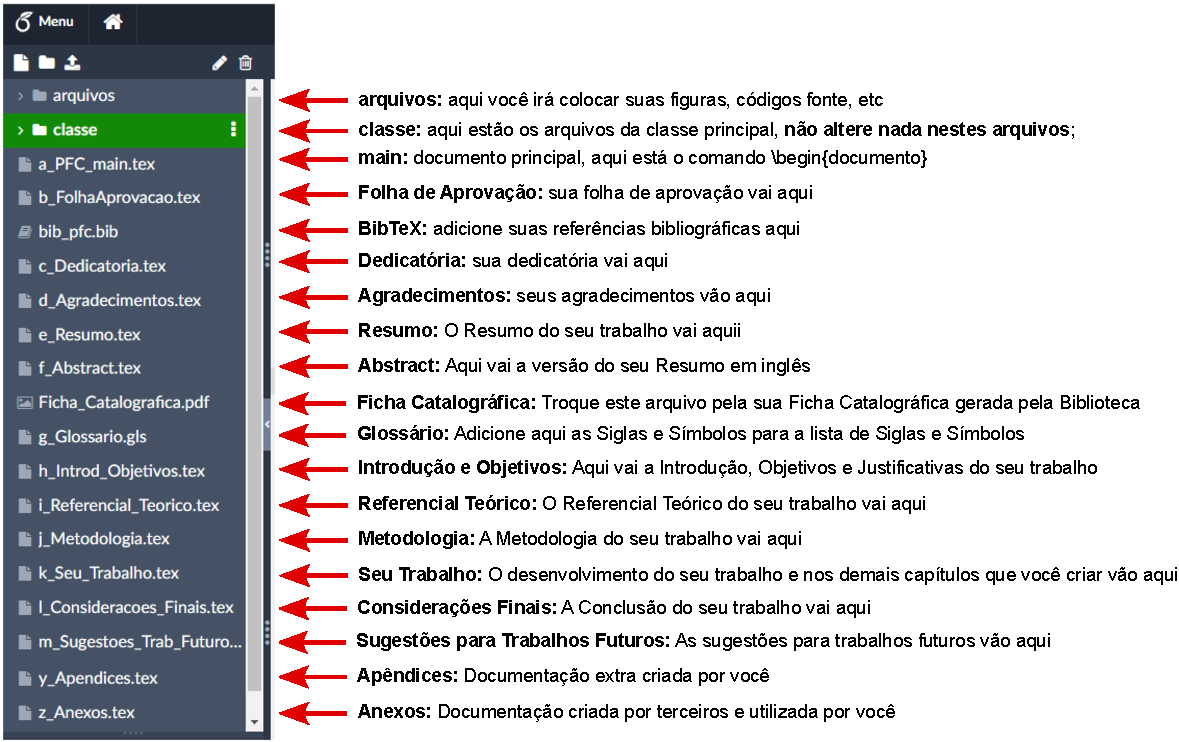
\includegraphics[width=14cm]{arquivos/arqcls/Organiza_template.pdf}
%      \caption{Organização deste Modelo ({\it template}) no Overleaf}
%      \label{fig:Organiza_Template}
%  \end{figure}

% \begin{CaixaVermelha}
%     \begin{enumerate}
%         \item {\bf IMPORTANTE:}  Não alterar nenhum documento dentro da pasta {\bf classe}. Os arquivos desta pasta possuem os comandos de formatação deste {\it template} que foi aprovado pelo colegiado da COEEL, logo não é permitido nenhuma alteração;
%         \item O conteúdo da pasta {\bf arquivos} pode ser alterado e modificado livremente;
%         \item O conteúdo da pasta {\bf arqcls} são as figuras e códigos exemplo deste modelo ({\it template});
%     \end{enumerate}
% \end{CaixaVermelha}
 

% %%%%%%%%%%%%%%%%%%%%%%%%%%%%%

% \section{Selecionar a classe para o modo de PFC ou modo de Relatório}

% Este Modelo ({\it template}) pode ser utilizado para a produção de Monografias de {\bf PFC (Projeto Final de Curso)} de Egenharia Elétrica, e também para {\bf Relatórios} de disciplinas.

% Para habilitar este modelo para funcionar como {\bf PFC}, altere o documento principal (Main) conforme mostra o código~\ref{cod:PFC}: 

% \ImportaCodigo[language=tex, caption=Para produzir PFC-Projeto Final de Curso, label=cod:PFC]{arquivos/arqcls/Cod_PFC.txt}

% Para habilitar este modelo para funcionar como {\bf Relatório de Disciplina}, altere o documento principal (Main) conforme mostra o código~\ref{cod:Relat}: 

% \ImportaCodigo[language=tex, caption=Para produzir Relatório de Disciplina, label=cod:Relat]{arquivos/arqcls/Cod_Relat.txt}

% %%%%%%%%%%%%%%%%%%%%%%%%%%%%%
% \pagebreak\clearpage\newpage

% \section{O que deve ser preenchido para a geração automática da parte Pré-Textual do seu trabalho}

% {\bf Para gerar automaticamente a Capa e Folha de Rosto:} Entre no documento principal (\verb|a_PFC_main.tex|), e procure pelos comandos listados abaixo, perceba que existem locais apropriados para preenchimento caso seja um PFC ou Relatório:

% \begin{itemize}
%     \item {\Large \verb|\Titulo{}|:} adicionar o título do seu trabalho aqui;
%     \item {\Large \verb|\Autor{}|:} preencha com o seu nome;
%     \item {\Large \verb|\Professor{}|:} preencha somente se for Relatório;
%     \item {\Large \verb|\Disciplina{}|:} preencha somente se for Relatório;
%     \item {\Large \verb|\Orientador{}|:} preencha somente se for PFC;
%     \item {\Large \verb|\Coorieantador{}|:} preencha somente se for PFC;
%     \item {\Large \verb|\DataDefesa{}|:} preencha com a data de defesa do PFC ou com a data de entrega do relatório, caso não saiba a data, deixe \verb|\today|;
%     \item {\Large \verb|\CidadeDefesa{}|:} a cidade sempre será Vitória da Conquista, pois trata-se da cidade onde se encontra a COEEL;
% \end{itemize}

% %%%%%%%%%%%%%%%%%%%%%%%%%%%%%
% \pagebreak\clearpage\newpage

% \section{Procedimentos da Biblioteca para solicitação da Ficha Catalográfica}
% \label{sec:Biblioteca}

% A ficha catalográfica é um serviço prestado pela Biblioteca. 

% Para confecção de Ficha Catalográfica, o bibliotecário segue as regras e normas
% internacionais do Código de Catalogação Anglo-Americano - 2ª edição (AACR2).

% {\bf PROCEDIMENTO:}

% A solicitação deverá ser feita quando o aluno já tiver apresentado seu trabalho para a Banca Examinadora e feito todas as correções sugeridas.

% As palavras-chave devem ser de três a cinco. Devem ser palavras que identifiquem o tema do trabalho que, isoladas, proporcionem ao leitor o entendimento do assunto do trabalho.

% {\bf PARA ONDE ENVIAR A SOLICITAÇÃO:}

% A solicitação para elaboração da ficha deverá ser feita exclusivamente por meio do e-mail da Biblioteca- \url{biblio.ifba.conquista@gmail.com}

% {\bf PRAZO DE RESPOSTA:}

% O prazo de resposta das solicitações (de ficha ou alteração de fichas já enviadas) é de até 06 (seis) dias "úteis" a depender da demanda do serviço. Por isso, recomendamos que não deixe seu pedido para a última hora, pois a demanda é alta em períodos de entrega da versão final.

% Fiz o meu pedido há mais de 6 dias e não tive respostas. O que fazer? Neste caso, entre em contato com a Biblioteca, pois pode ter tido algum problema no recebimento do e-mail.

% {\bf OUTRAS INFORMAÇÕES:}

% Os usuários com pendência na Biblioteca não poderão solicitar o serviço;

% A ficha catalográfica deverá estar localizada na parte inferior do verso da folha de rosto, de forma centralizada no trabalho impresso e também deve constar no trabalho em formato digital;

% A ficha catalográfica deve ser anexada na íntegra, ou seja, não é permitido ``recortar'' ou omitir informações disponíveis no documento, e não deve ser alterada sem permissão do bibliotecário;

% As fichas catalográficas são enviadas no formato de arquivo não editável para garantir a formatação da peça. Se o solicitante identificar erros de digitação ou de inserção de
% dados pode solicitar a biblioteca a correção dos erros;

% A ficha catalográfica deverá ser inserida na parte inferior do verso da Folha de Rosto do trabalho. A folha da ficha catalográfica deve ser contada para a paginação, mas não numerada, por ser um elemento pré-textual.

% De acordo com a Resolução n. 184, de 29 de setembro de 2017, do Conselho
% Federal de Biblioteconomia (CFB), a ficha catalográfica deve estar acompanhada do
% nome e do número de registro profissional do bibliotecário que a elaborou. Portanto,
% solicitamos que as informações da ficha não sejam alteradas. Se necessitar de qualquer alteração na ficha, por favor, solicite-a a bibliotecária.

% %%%%%%%%%%%%%%%%%%%%%%%%%%%%

% \subsection{Como adicionar automaticamente o PDF da Ficha Catalográfica}

% Após sua defesa do PFC perante a banca avaliadora, caso seu trabalho tenha sido aprovado, você realizará as correções sugeridas pela banca e pelo seu orientador.

% Após aprovação do texto você precisará solicitar a Ficha Catalográfica para a Biblioteca do campus, conforme orientações da seção~\ref{sec:Biblioteca} da página~\pageref{sec:Biblioteca}.

% Para acrescentar automaticamente o PDF da Ficha Catalográfica fornecida pela Biblioteca no seu documento, abra o documento principal {\bf a\_PFC\_main.tex} e procure pela parte que trata sobre a Ficha Catalográfica, como mostra o código~\ref{cod:FichaCatalografica} a seguir.

% Faça upload do PDF da sua Ficha Catalográfica no ~\LaTeX~Overleaf~ e substitua o arquivo PDF chamado: \verb|Ficha_Catalografica.pdf| pela sua Ficha Catalográfica, e caso o nome do PDF seja diferente, renomeie o nome do PDF no código~\ref{cod:FichaCatalografica}. Desta forma o ~\LaTeX~ irá importar e adicionar sua Ficha Catalográfica automaticamente no seu documento.

% \pagebreak

% \begin{Codigo}[language=tex, caption=Código da Ficha Catalográfica no documento principal {\bf a\_PFC\_main.tex}, label=cod:FichaCatalografica]
%     %%%%%%%%%%%%%%%%%%%%%%%%%%%%
%     %%%% FICHA CATALOGRAFICA
%     % apenas para PFC
%     %
%     \ifbool{pfc}{ 
%         \newpage\clearpage\pagebreak
%         \ifpdf\phantomsection\fi
%         \addcontentsline{toc}{chapter}{Ficha Catalografica}
%         % inclua o PDF da ficha catalografica 
%         % feita pela biblioteca
%         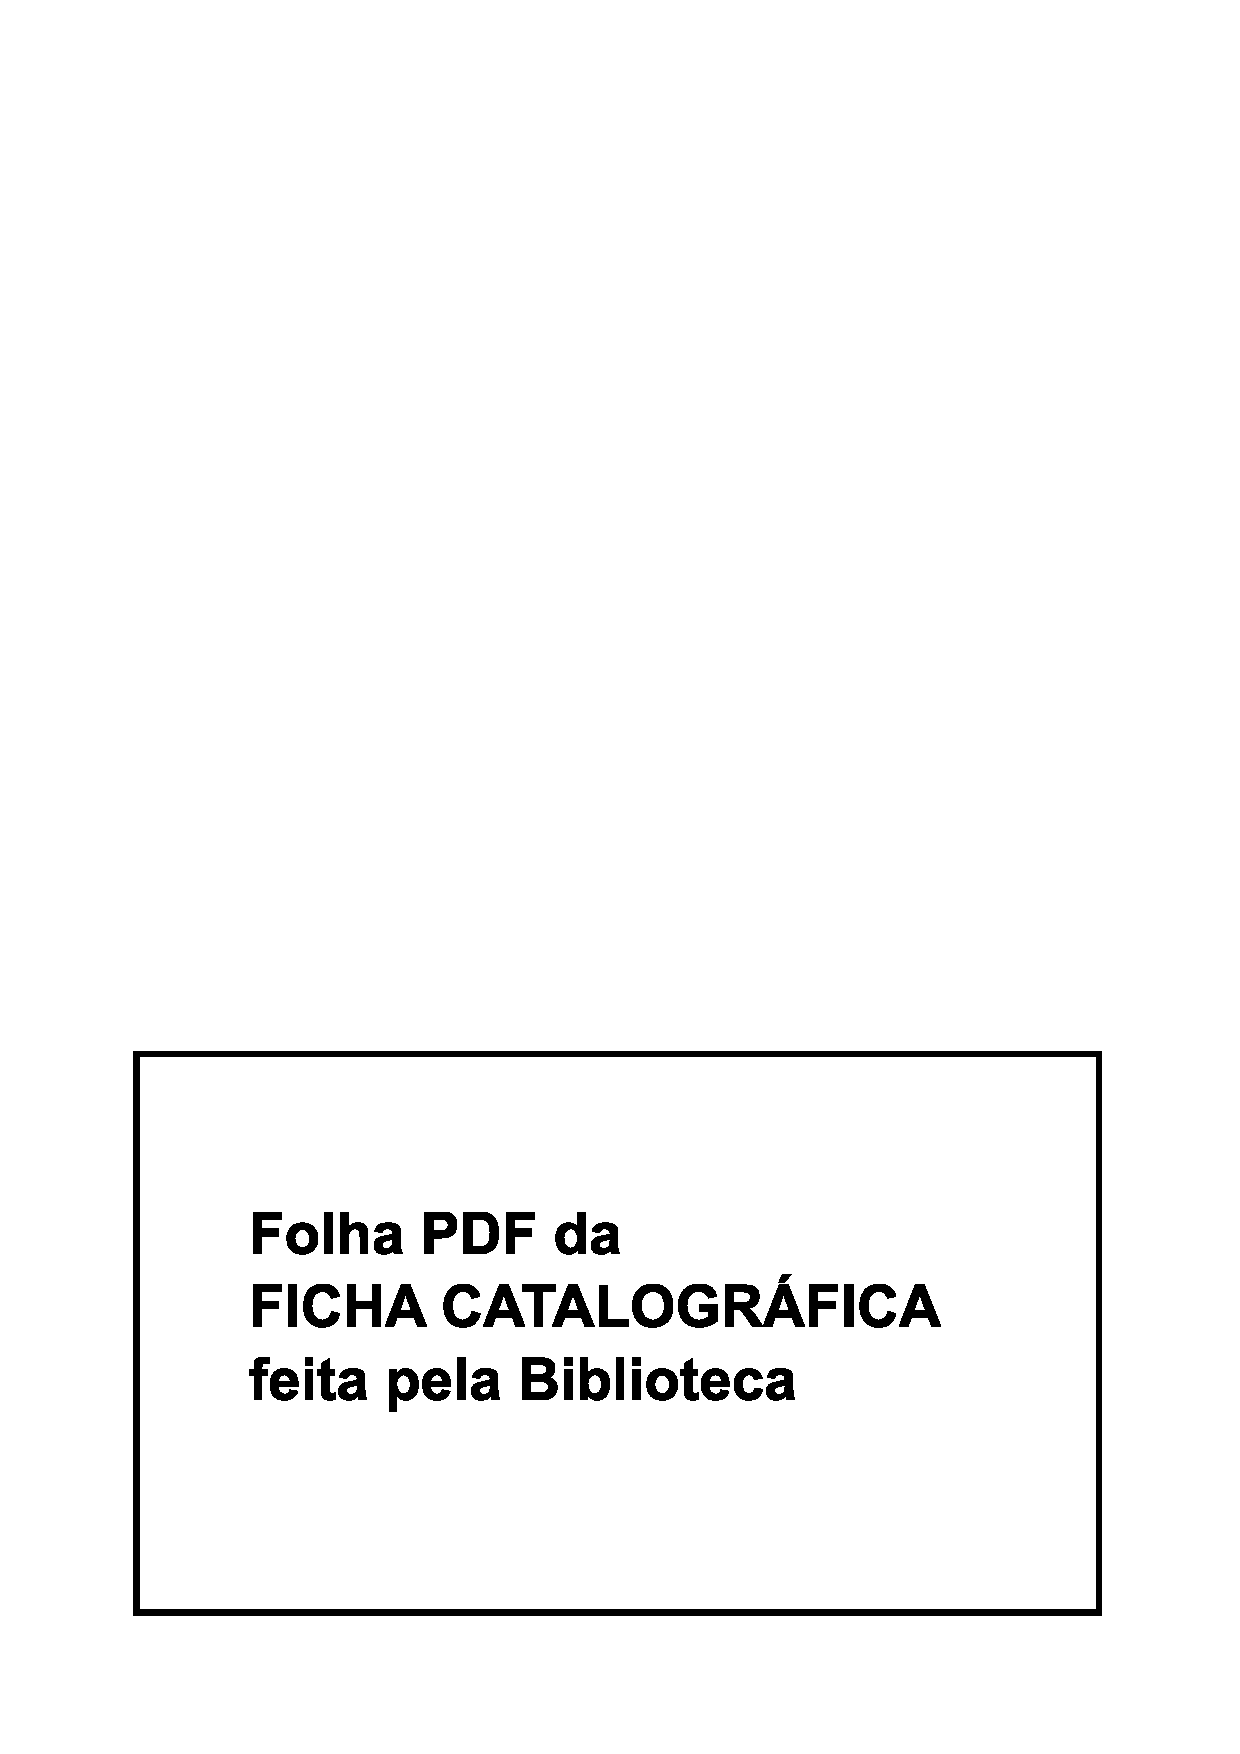
\includepdf[pages=1]{Ficha_Catalografica.pdf}
%     }{}
% \end{Codigo}

% %%%%%%%%%%%%%%%%%%%%%%%%%%%%%%

% \section{Adicionando automaticamente o PDF da Folha de Aprovação}

% Verifique o documento chamado \verb|b_FolhaAprovacao.tex|. 

% Caso a Folha de Aprovação de seu trabalho precise ser assinada manualmente, à caneta, preencha o nome, titulação e campus dos membros da banca, imprima esta folha PDF e a leve no dia de sua defesa para que a banca possa assiná-la à caneta, depois você irá escaneá-la e adicioná-la da mesma forma que se adiciona a Folha de Aprovação assinada digitalmente, no documento principal \verb|a_PFC_main.tex|, conforme mostra o código~\ref{cod:FolhaAprovacao}.

% Caso a Folha de Aprovação de seja assinada digitalmente pelo sistema SEI ou pelo SOU.GOV, seu orientador irá providenciar a confecção da Folha de Aprovação e providenciará a assinatura dos membros da banca e você irá adicioná-la ao seu trabalho, no documento \verb|a_PFC_main.tex| da conforme mostra o código~\ref{cod:FolhaAprovacao}. Renomeie o PDF da sua Folha de Aprovação assinada para \verb|Folha_Aprovacao.pdf| e faça o upload do PDF para o ~\LaTeX~Overleaf. 

% \pagebreak

% \begin{Codigo}[language=tex, caption=Código da Folha de Aprovação no documento principal {\bf a\_PFC\_main.tex}, label=cod:FolhaAprovacao]
%     %%%%%%%%%%%%%%%%%%%%%%%%%%%%
%     %%%% FOLHA DE APROVACAO
%     % Apenas para PFC
%     %
%     \ifbool{pfc}{ 
%         \newpage\clearpage
%         \ifpdf\phantomsection\fi
%         \addcontentsline{toc}{chapter}{Folha de Aprovacao}
    
%         \includepdf[pages=1]{Folha_Aprovacao.pdf} 

%         % comente esta linha quando 
%         % for anexar o PDF
%         % %%%%%%%%%%%%%%%%%%%%%%%%%%%%%%%%%%%%%%%%%%%%%
%%%%%% FOLHA DE APROVAÇÃO
%%%%%%%%%%%%%%%%%%%%%%%%%%%%%%%%%%%%%%%%%%%%%

% caso queira incluir o PDF da folha de aprovação assinada digitalmente pelos membros da banca pelo SEI ou pelo SOU.GOV, acrescente o arquivo PDF utilizando o comando seguinte comando dentro do arquivo MAIN:
% \includepdf[pages=1]{Folha_Aprovacao.pdf} % descomente esta linha se for anexar o PDF

  \clearpage\newpage\pagebreak%
  \pagestyle{plain}
  \begin{center}%
    \textbf{\Large \@Titulo  }\\%
    \vspace{1.2cm}%
    \MakeUppercase{\textbf{\Large \@Autor}}\\%
  \end{center}%
  \vspace{0.6cm}%

  A presente Monografia, apresentada em sessão realizada em \textbf{ \@DataDefesa}, foi avaliada como adequada para a obtenção do Grau de Bacharel em Sistemas de Informação, julgada \textbf{aprovada} em sua forma final pela Coordenação do Curso de Sistemas de Informação do Instituto Federal de Educação, Ciência e Tecnologia da Bahia, \textit{campus} Vitória da Conquista.

  \begin{center}
    
    \vspace{7mm}
    Vitória da Conquista/BA, \@DataDefesa.
    \vspace{7mm}
    \vspace{7mm}
    \rule[0cm]{10cm}{0,5mm}\\
    \textbf{}
    Prof. Me. Alexandro dos Aantos Silva\\
    (Coordenador do Curso - IFBA campus Vitória da Conquista)\\
    \vspace{7mm}
    \textbf{\small BANCA EXAMINADORA:}\par
    \vspace{7mm}
    \rule[0cm]{10cm}{0,5mm}\\
    Prof. DSc. Djan Almeida Santos (Orientador)\\
    IFBA campus Vitória da Conquista\\
    \vspace{7mm}
    \rule[0cm]{10cm}{0,5mm}\\
    Prof. Msc. Crijina Chagas Flores\\
    IFBA campus Vitória da Conquista\\

    \vspace{7mm}
    \rule[0cm]{10cm}{0,5mm}\\
    Prof. Msc. Liojes de Oliveira Carneiro\\
    IFBA campus Vitória da Conquista\\
    
  \end{center}
  
  
  % \vfill % leva para o botton da página
  % \begin{center}%    
  %   {\large  \@CidadeDefesa}\\%
  %   \vspace{1mm}%
  %   {\large  \@DataDefesa }%
  % \end{center}%
 
%     }{}
% \end{Codigo}

% %%%%%%%%%%%%%%%%%%%%%%%%%%%%%

% \section{Glossário: Comando ``gls'' para  gerar automaticamente lista de Símbolos e Siglas}
% \label{sec:Glossario}

% Verifique que existe um documento chamado: \verb|g_Glossario.tex|, abra este documento e verifique que este documento é uma Biblioteca de Lista de Siglas e Símbolos. Preencher este documento com as Siglas e com os Símbolos utilizados no seu documento.

% Abra e veja o código~\ref{cod:Glo1}, você irá preencher o {\bf apelido} com um apelido para a sigla ou símbolo que será citado; preencher o {\bf name} com o nome da sigla ou símbolo que irá aparecer no texto; preencher o {\bf description} com a descrição do que é a sigla ou símbolo. Note que em alguns casos o {\bf apelido} e o {\bf name} poderão ser iguais.

% \pagebreak

% \begin{Codigo}[language=tex, caption=Biblioteca de Glossários~ {\bf g\_Glossario.gls}, label=cod:Glo1]
%    \newglossaryentry{apelido} 
%     {
%     name = {Nome que aparece no texto},
%     description = {Descricao da sigla ou simbolo}
%     }
% \end{Codigo}

% Vamos dar um exemplo de como preencher o \verb|g_Glossario.tex| e como citar no texto as siglas e símbolos. Supondo que queremos colocar no glossário a sigla IEEE e que sua descrição seja: IEEE - Instituto de Engenheiros Eletricistas e Eletrônicos (IEEE is the world's largest technical professional organization dedicated to advancing technology for the benefit of humanity) e queremos citar a sigla $cos(\varphi)$ com descrição de {Fator de Potência} podemos adicionar o seguinte código no documento \verb|g_Glossario.gls|, como mostra o código~\ref{cod:Glo2}:

% \begin{Codigo}[language=tex, caption=Biblioteca de Glossários~ {\bf g\_Glossario.gls}, label=cod:Glo2]
%     % para SIGLAS
%     \newglossaryentry{IEEE} % 
%     {
%     name = {IEEE},
%     description = {IEEE - Instituto de Engenheiros
%     Eletricistas e Eletronicos (IEEE is the world's 
%     largest technical professional organization 
%     dedicated to advancing technology for the benefit 
%     of humanity)}
%     }
%     % para SIMBOLOS
%     \newglossaryentry{FP}
%     {
%     name = {$cos(\varphi)$},
%     description = {Fator de Potencia}
%     }
% \end{Codigo}

% \begin{CaixaVermelha}
%     Para que as siglas e símbolos apareçam no glossário, obrigatoriamente elas deverão ser citadas no texto.
% \end{CaixaVermelha}

% Para citarmos no texto as siglas e símbolos que adicionamos no documento \verb|g_Glossario.gls|, precisamos utilizar o comando \verb|\gls{}|, como por exemplo estou citando o \gls{IEEE} com o comando \verb|\gls{IEEE}| e o símbolo \gls{FP} com o comando \verb|\gls{FP}| no meu texto e automaticamente eles aparecerão no glossário. 

% Note que as citações \gls{IEEE} e \gls{FP} aparecem na forma de links que ao serem clicados apontam para o glossário, que informa a notação, a descrição e as páginas onde as siglas e símbolos se encontram no texto.

% %%%%%%%%%%%%%%%%%%%%%%%%%%%%%

% \section{Comando ``index'' para gerar automaticamente o Índice Remissivo}

% O Índice Remissivo não é obrigatório, é apenas mais um artifício que completa seu texto, no qual as palavras referenciadas aparecem no final do seu trabalho, em ordem alfabética com o número da página onde elas se encontram.

% Caso você queira acrescentar alguma palavra no Índice Remissivo, você precisará utilizar o comando \verb|\index{}|, como por exemplo iremos adicionar as seguintes frutas no índice remissivo: abacate~\index{abacate}, banana~\index{banana}, cereja~\index{cereja}, cajá~\index{cajá}, caqui~\index{caqui}, jabuticaba~\index{jabuticaba} e os seguintes objetos: carro~\index{carro}, sofá~\index{sofá}, brinquedo~\index{brinquedo}, mercadoria~\index{mercadoria}, vidro~\index{vidro}, jarro~\index{jarro}, alfinete~\index{alfinete}.

% %%%%%%%%%%%%%%%%%%%%%%%%%%%%%
% \newpage\clearpage\pagebreak

% \section{Como adicionar códigos de linguagens de programação no texto, colorindo os comandos de sintaxe}

% A classe \verb|cls-PFC-COEEL.cls| está configurada para aceitar duas formas de acrescentarmos códigos fonte em nossos textos.

% A {\bf forma direta} consiste em adicionar o código diretamente aqui no texto utilizando o comando \verb|\begin{Codigo} ... \end{Codigo}|, com a palavra Codigo com a letra C maiúscula, conforme mostra o exemplo~\ref{cod:CodDireta}.

% \begin{Codigo}[language=tex, caption=Forma direta de acrescentar Códigos no texto, label=cod:CodDireta]
%     \begin{codigo}[language=Nome da Linguagem,
%         caption=Titulo do Codigo,
%         label=cod:LabelCodigo]
%             %
%             %  Seu codigo vem aqui
%             %
%     \end{codigo}
% \end{Codigo}

% Vamos dar um exemplo prático de utilização de um código em linguagem Python colocando o código diretamente no texto, conforme mostra o código~\ref{cod:CodPython}. Perceba que as palavras reservadas da linguagem Python foram coloridas.

% \begin{Codigo}[language=Python, caption=Programa em Python para Somar Dois Números, label=cod:CodPython]
%     # exemplo de codigo linguagem  Python para
%     # somar dois numeros
%     num1 = float(input('Digite o primeiro numero: '))
%     num2 = float(input('Digite o segundo numero: '))

%     soma = num1 + num2

%     print('A soma de {} e {} = {}'.format(num1,num2,soma))
% \end{Codigo}

% A segunda é a {\bf forma de importação de arquivo}, que consiste em chamarmos o arquivo contendo o código fonte com o comando: \verb|\ImportaCodigo|, como mostra o código~\ref{cod:Codimporta}.

% \begin{Codigo}[language=tex, caption=Forma de importar Códigos para o texto, label=cod:Codimporta]
%     \ImportaCodigo[language=Nome da Linguagem,
%         caption=Titulo do Codigo,
%         label=cod:LabelCod]
%         {caminho do codigo.cpp}
% \end{Codigo}

% Vamos ao exemplo prático de utilização da forma de importação de arquivos: veja que na pasta {\bf arquivos} existe um documento com o nome \verb|codigo_exemplo.cpp|. Abra este arquivo e verá um exemplo de código em C++ para a soma de dois números, conforme mostra o código~\ref{cod:CodCpp}.

% \ImportaCodigo[language=C++,
%     caption=Código para a Soma de Dois Números em C++,
%     label=cod:CodCpp]
%     {arquivos/codigo_exemplo.cpp}


% \pagebreak
% ~
% \vspace{8mm}

% Perceba que a sintaxe do código~\ref{cod:Codimporta2} que foi utilizada para gerar o código~\ref{cod:CodCpp} com a forma de {\bf importação de arquivos} é mais enxuta, e ao meu ver é melhor.    


% \vspace{5mm}
% \begin{Codigo}[language=tex, caption=Forma de importar Códigos para o texto, label=cod:Codimporta2]
%     \ImportaCodigo[language=C++,
%         caption=Codigo para a Soma de Dois Numeros em C++,
%         label=cod:CodCpp]
%         {arquivos/codigo_exemplo.cpp}
% \end{Codigo}

% \vspace{0.6cm}
% \begin{CaixaVermelha}
%      \begin{enumerate}
%          \item Os comandos para inserção de códigos no texto não aceitam palavras acentuadas, nesse sentido você precisará retirar os acentos do seu código para poder citá-los no texto.
%         \item Pequenos trechos de código podem e devem ser citados ao longo do texto, porém códigos grandes devem vir nos Apêndices (quando for de sua autoria), ou nos Anexos (quando for de autoria de terceiros).
%      \end{enumerate}
% \end{CaixaVermelha}

% %%%%%%%%%%%%%%%%%%%%%%%%%%%%%%


% \section{Adicionar Figuras, Gráficos, Tabelas, E-quações e Caixas Coloridas no texto}

% \subsection{Figuras}

% Para adicionarmos figuras no texto veja a sintaxe do código~\ref{cod:Figs} e o resultado no código~\ref{fig:LogoIFBAh} da página~\pageref{fig:LogoIFBAh},  repare que a figura deve vir centralizada no texto e com o título na parte de baixo, e a fonte de onde foi retirada a figura deve vir na lateral (comando \verb|\FonteFig{}|) e deve ser citada nas Referências. Para citar as figuras, utilizamos o comando \verb|~\ref{}| e para citar a página utilizamos o comando \verb|~\pageref{}|.

% \newpage\clearpage\pagebreak

% \begin{Codigo}[language=tex, 
%     caption=Sintaxe para adicionar Figuras no Texto, 
%     label=cod:Figs]
%  \begin{figure}[htb]
%    \centering
%    
\includegraphics[width=15cm]{arquivos/LogoIFBA-VDC-h.pdf}
%    \FonteFig{Reitoria do IFBA}
%    \caption{Logomarca horizontal do IFBA campus Vitoria 
%    da Conquista}
%    \label{fig:LogoIFBAh}
%  \end{figure}
% \end{Codigo}

% \begin{figure}[htb]
%     \centering
%     
\includegraphics[width=15cm]{arquivos/LogoIFBA-VDC-h.pdf}
%     \FonteFig{Reitoria do IFBA \cite{LogoIFBA_pagina}}
%     \caption{Logomarca horizontal do IFBA campus Vitória da Conquista}
%     \label{fig:LogoIFBAh}
% \end{figure}

% \vspace{2cm}

% \begin{CaixaVerde}
%     \begin{itemize}
%         \item Dê preferência para figuras no formato vetorizado, como: PDF ou EPS. Para fotos os formatos JPG e PNG são compatíveis;
%         \item Figuras com qualidade ruim empobrecem seu trabalho;
%         \item A fonte das figuras devem ser citadas nas referências quando não forem feitas pelo próprio autor.
%         \end{itemize}
% \end{CaixaVerde}

% \vspace{5mm}

% Segue um exemplo de 2 figuras lado a lado: Ver a primeira figura em~\ref{fig:LogoCOEEL2} e a segunda figura em~\ref{fig:LogoCOEEL3}.
% A caixa em volta da figura realizada pelo comando \verb|\fbox{}| é facultativa.

% ~
% \vspace{5mm}

% % Duas figuras lado a lado
% \begin{figure}[htb] 
%     \FonteFig{Colegiado da COEEL}
%     \begin{minipage}[b]{0.44 \linewidth}
%         \fbox{
\includegraphics[width=\linewidth]{arquivos/LogoCOEEL.pdf}}
%             \caption{Logomarca da COEEL}
%             \label{fig:LogoCOEEL2}
%     \end{minipage}
%     \hfill
%     \begin{minipage}[b]{0.44 \linewidth}
%         \fbox{
\includegraphics[width=\linewidth]{arquivos/LogoCOEEL.pdf}}
%         \caption{Logomarca da COEEL}
%         \label{fig:LogoCOEEL3}         
%     \end{minipage} 
%     \FonteFig{Colegiado da COEEL}    
% \end{figure}

% ~

% Segue o código~\ref{cod:Figs2a2} de como colocar 2 figuras lado a lado. Lembrando que o comando \verb|\fbox{}| é opcional.

% Não se esqueça da fonte de referências das figuras, é obrigatório citar onde foram retiradas as figuras, caso seja você mesmo quem as construiu, cite como: Próprio autor.

% \begin{Codigo}[language=tex, 
%     caption=Sintaxe para adicionar 2 Figuras lado a lado no Texto, 
%     label=cod:Figs2a2]
% % Duas figuras lado a lado
% \begin{figure}[htb] 
%   \FonteFig{Colegiado da COEEL}
%   \begin{minipage}[b]{0.44 \linewidth}
%      \fbox{\includegraphics[width=\linewidth]
%           {arquivos/LogoCOEEL.pdf}}
%      \caption{Logomarca da COEEL}
%      \label{fig:LogoCOEEL2}
%   \end{minipage}
%   \hfill
%   \begin{minipage}[b]{0.44 \linewidth}
%     \fbox{\includegraphics[width=\linewidth]
%          {arquivos/LogoCOEEL.pdf}}
%     \caption{Logomarca da COEEL}
%     \label{fig:LogoCOEEL3}         
%   \end{minipage} 
%   \FonteFig{Colegiado da COEEL}    
% \end{figure}
% \end{Codigo}

% %%%%%%%%%%%%%%%%%%%%%%%%%%%%%%%
% \pagebreak

% \subsection{Gráficos}

% Os gráficos são adicionados no texto como figuras, conforme~\ref{fig:GraficoFP}. Dê preferência para figuras vetorizadas (PDF ou EPS).

% \begin{figure}[htb]
%     \centering
%     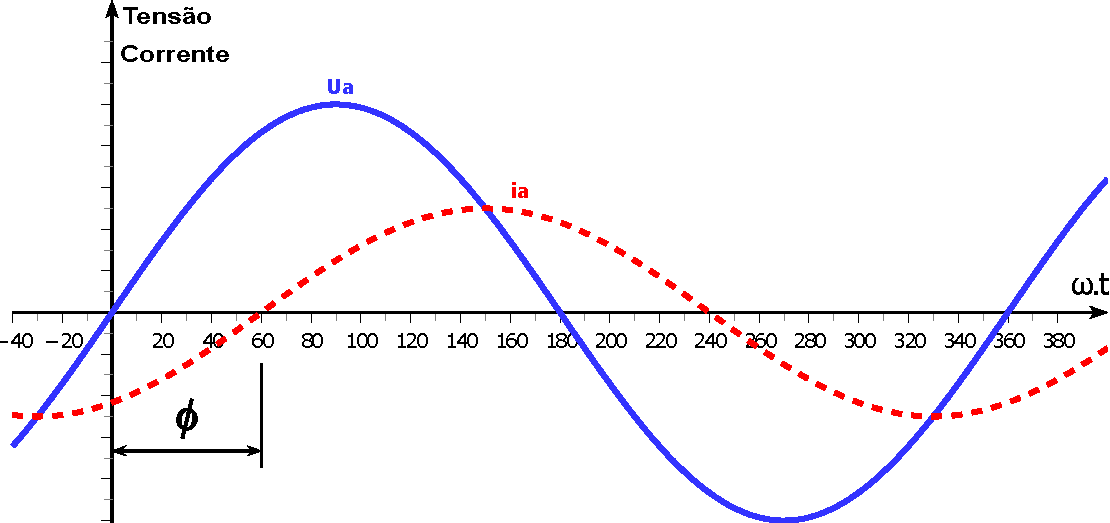
\includegraphics[width=15.3cm]{arquivos/GraficoFP.pdf}
%     \FonteFig{Próprio Autor}
%     \caption{Curvas de Tensão e Corrente em Carga Indutiva com Ângulo~$\phi$ de Fator de Potência}
%     \label{fig:GraficoFP}
% \end{figure}  

% Legenda:\\
% \vspace{-1.3cm}
% \begin{tabbing}
%     \hspace{1cm}  \= \hspace{1cm} \= \kill \\
%     \gls{Ua}      \> $\Rightarrow$ \> Tensão na Fase A ~~~(\textcolor{blue}{\rule{3cm}{1mm}}); \\
%     \gls{Ia}      \> $\Rightarrow$ \> Corrente na Fase A (\textcolor{red}{\hdashrule[0.1ex]{3.1cm}{1mm}{2mm}}); \\
%     \gls{fi}    \> $\Rightarrow$ \> Ângulo do Fator de Potência; \\
%     \gls{w}    \> $\Rightarrow$ \> Velocidade angular: $\omega=2\cdot \pi \cdot f$;    
% \end{tabbing}

% \begin{itemize}
%     \item \verb|\rule{tamanho}{espessura}| cria uma linha com tamanho e espessura definidos. 
%     \item \verb|\hdashrule[0.1ex]{tamanho}{espessura}{distancia entre os tracos}}| cria uma linha tracejada com tamanho, espessura e distância entre os traços definidos.
% \end{itemize}

% \begin{CaixaVerde}
%     Perceba que a legenda possui o comando \verb|\gls{}| que adiciona os símbolos no Glossário. Para criar um glossário, veja a seção~\ref{sec:Glossario} na página~\pageref{sec:Glossario}.
% \end{CaixaVerde}

% \pagebreak
% \begin{Codigo}[language=tex, 
%     caption=Sintaxe para criar a legenda alinhada e com citação no Glossário, 
%     label=cod:LegendaGraf]
% \begin{tabbing}
%   \hspace{1cm}  \=  \hspace{1cm}   \= \kill \\
%   \gls{Ua}      \>  $\Rightarrow$  \> Tensao na Fase A
%                     (\textcolor{blue}{\rule{3cm}{1mm}}); \\
%   \gls{Ia}      \>  $\Rightarrow$  \> Corrente na Fase A
%     (\textcolor{red}{\hdashrule[0.1ex]{3.1cm}{1mm}{2mm}}); \\
%   \gls{fi}      \>  $\Rightarrow$  \> Angulo do Fator de
%                                       Potencia;  \\   
% \end{tabbing}
% \end{Codigo}

% %%%%%%%%%%%%%%%%%%%%%%%%%%%%%%%
% %\pagebreak

% \subsection{Tabelas}

% Para adicionarmos tabelas no texto veja a sintaxe do código~\ref{cod:Tab} na página~\pageref{cod:Tab} e o resultado na tabela~\ref{tab:Tabela} ,  repare que a tabela deve vir centralizada no texto e com o título na parte de cima, e a fonte de onde foi retirada a tabela (comando \verb|\FonteTab{}|) deve vir na parte de baixo, e deve ser citada nas Referências. 

% As tabelas devem ser enxutas, e devem conter somente as linhas de Cima, Meio e de Baixo, sendo que não se utiliza de linhas de coluna, nem linhas separadoras entre linhas.

% \begin{CaixaVermelha}
%     \begin{enumerate}
%         \item Textos de palavras devem vir justificados a esquerda, para ficarem  alinhados a esquerda na coluna;
%         \item Números devem vir justificados a direita, sendo que todos os números de uma mesma coluna devem vir com o mesmo número de casas decimais para alinhamento com {\bf vírgula debaixo de vírgula na coluna}.
%     \end{enumerate}
% \end{CaixaVermelha}

% \begin{table}[htb]
%     \centering
%     \caption{Note que as palavras são alinhadas à esquerda e os números são alinhados à direita e com vírgula debaixo de vírgula}
%     \begin{tabular}{lrr}
%        \Linha % linha grossa
%        {\bf Números} & {\bf 4 Casas} & {\bf Aleatórios} \\
%        \hline % linha fina      
%        Número $\pi$          &    3,1416  &    125,07  \\
%        Núm. de Euler $e$     &    2,7182  &     79,00  \\
%        Núm. de Ouro $\phi$   &    1,6180  &  1.975,23  \\
%        Raiz: $\sqrt{2}$            &    1,4142  &      8,91  \\ 
%        Raiz: $\sqrt{3}$            &    1,7320  &    543,10  \\
%        \Linha % linha grossa
%     \end{tabular}    
%     \FonteTab{Cite aqui a fonte da tabela}
%     \label{tab:Tabela}
% \end{table}

% Para alinhamento das células na coluna utilize a letra L minúscula (left) para alinhamento à esquerda, e utilize a letra R minúscula (right) para alinhamento à direita.


% \pagebreak
% Utilize o comando \verb|\Linha| para as linhas horizontais grossas e o comando \verb|\hline| para as linhas horizontais finas. 

% As linhas da vertical devem ser evitadas para que a tabela fique a mais limpa possível.

% \begin{Codigo}[language=tex, 
%     caption=Sintaxe para adicionar Tabelas no Texto, 
%     label=cod:Tab]
% \begin{table}[htb]
%     \centering
%     \caption{Note que as palavras sao alinhadas a esquerda 
%     e os numeros sao alinhados a direita e com 
%     virgula debaixo de virgula}
%     \begin{tabular}{lrr}
%        \Linha % linha grossa
%        {\bf Numeros}   & {\bf 4 Casas} & {\bf Aleatorios} \\
%        \hline % linha fina
%        Numero $\pi$        &    3,1416     &    125,07  \\
%        Euler $e$           &    2,7182     &     79,00  \\
%        Ouro $\phi$         &    1,6180     &  1.975,23  \\ 
%        Raiz: $\sqrt{2}$    &    1,4142     &      8,91  \\ 
%        Raiz: $\sqrt{3}$    &    1,7320     &    543,10  \\
%        \Linha % linha grossa
%     \end{tabular}    
%     \FonteTab{Cite aqui a fonte da tabela}
%     \label{tab:Tabela}
% \end{table}
% \end{Codigo}

% Para citar as tabelas, utilizamos o comando \verb|~\ref{}| e para citar a página utilizamos o comando \verb|~\pageref{}|.

% \subsubsection{Tabelas coloridas (opcional)} 

% De forma opcional você poderá colorir as células das linhas da tabela, conforme mostra a tabela~\ref{tab:TabelaColorida}.

% \begin{table}[htb]
%     \centering
%     \caption{Veja o alinhamento das palavras e números}
%     % colore a partir da segunda linha de vermelho e verde
%     \rowcolors{2}{red!20}{green!20}
%     \begin{tabular}{lrlrr}
%        \Linha % linha grossa
%        \rowcolor{red!60} % colore a linha imediatamente abaixo
%        \textbf{Fruta} & \textbf{Peso (kg)} & \textbf{Qualid.} & \textbf{R\$/kg}  &  \textbf{Total (R\$)}\\
%        \Linha % linha grossa
%        Maçã          & 1,250  & madura &  12,99  &  16,24 \\
%        Banana Prata  & 2,510  & verde  &   8,99  &  22,56 \\
%        Uva Niágara   & 1,860  & verde  &   7,09  &  13,19 \\
%        Pera          & 2,110  & madura &  12,67  &  26,73 \\
%        Kiwi          & 3,640  & verde  &  10,67  &  38,84 \\
%        Manga Palmer  & 5,300  & madura &   5,98  &  31,69 \\
%        \Linha % linha grossa
%        \rowcolor{green!60} % colore a linha imediatamente abaixo
%        \textbf{TOTAL} &       &        &         & {\bf 149,26} \\
%        \Linha % linha grossa
%     \end{tabular}    
%     \FonteTab{Cite aqui a fonte da tabela}
%     \label{tab:TabelaColorida}
% \end{table}

% \begin{itemize}
%     \item \verb|\rowcolor{nome da cor}|: colore a linha imediatamente abaixo do comando;
%     \item \verb|\rowcolors{num da linha}{nome da cor 1}{nome da cor 2}|: colore as linhas alternadas com a ``cor~1'' e ``cor~2'', a partir da linha especificada em ``num~da~linha'';
%     \item \verb|{green!20}|: colore com 20\% da cor verde, aumente este valor para cores mais escuras;
% \end{itemize}

% \vspace{5mm}

% O código~\ref{cod:Tab2} mostra como criar tabelas com linhas coloridas. Lembrando que colorir linhas é opcional.

% \pagebreak

% \begin{Codigo}[language=tex, 
%     caption=Sintaxe para adicionar Tabelas Coloridas no Texto, 
%     label=cod:Tab2]
% \begin{table}[htb]
%   \centering
%   \caption{Veja o alinhamento das palavras e numeros}
%   % colore a partir da segunda linha de vermelho e verde
%   \rowcolors{2}{red!20}{green!20}
%   \begin{tabular}{lrlrr}
%     \Linha % linha grossa
%     \rowcolor{red!60} % colore a linha imediatamente abaixo
%     \textbf{Fruta} & \textbf{Peso (kg)} & \textbf{Qualid.} &
%     \textbf{R\$/kg}  &  \textbf{Total (R\$)}\\
%     \Linha % linha grossa
%     Maca          & 1,250  & madura &  12,99  &  16,24 \\
%     Banana Prata  & 2,510  & verde  &   8,99  &  22,56 \\
%     Uva Niagara   & 1,860  & verde  &   7,09  &  13,19 \\
%     Pera          & 2,110  & madura &  12,67  &  26,73 \\
%     Kiwi          & 3,640  & verde  &  10,67  &  38,84 \\
%     Manga Palmer  & 5,300  & madura &   5,98  &  31,69 \\
%     \Linha % linha grossa
%     \rowcolor{green!60} % colore a linha imediatamente abaixo
%     \textbf{TOTAL} &    &     &      & {\bf 149,26} \\
%     \Linha % linha grossa
%   \end{tabular}    
%   \FonteTab{Cite aqui a fonte da tabela}
%   \label{tab:TabelaColorida}
% \end{table}

% \end{Codigo}

% %%%%%%%%%%%%%%%%%%%%%%%%%%%%%%%
% \pagebreak\clearpage\newpage

% \subsection{Equações}

% Para adicionar equações no texto, utiliza-se a sintaxe normal do ~\LaTeX, o comando \verb|\begin{equation}|, conforme mostra a equação~\ref{eq:NumEsp}, lembrando que os símbolos devem possuir legenda próxima à equação, e devem ser adicionadas também no glossário:

% \begin{equation}
%     N_1 = \frac{\sqrt{2}}{2 \cdot \pi } \cdot \frac{U_1 \cdot  10^8}{f \cdot S_L \cdot B} \quad \Rightarrow \quad N_1 = \frac{U_1 \cdot 10^8}{4,44 \cdot f \cdot S_L \cdot B}
%     \label{eq:NumEsp}
% \end{equation}

% Sendo que:\\
% \vspace{-1.5cm}
% \begin{tabbing}
%     \hspace{1cm}  \= \hspace{1cm} \= \kill \\
%     \gls{N1}      \> $\Rightarrow$ \> Número de espiras do primário; \\
%     \gls{U1}      \> $\Rightarrow$ \> Tensão do primário (V); \\
%     \gls{freq}    \> $\Rightarrow$ \> frequência (Hz); \\
%     \gls{SL}      \> $\Rightarrow$ \> Área da Seção Líquida do núcleo ($cm^2$); \\
%     \gls{DenFlux} \> $\Rightarrow$ \> Densidade de Fluxo Magnético (G = Gauss); 
% \end{tabbing}

% \vspace{4mm}
% \begin{CaixaVermelha}
%     Todas as equações precisam ser numeradas e citadas ao longo do texto, bem como devem possuir a legenda dos símbolos (abaixo da equação) quando a equação aparece pela primeira vez no texto.
% \end{CaixaVermelha}

% %\pagebreak\newpage\clearpage

% O código para gerar a equação~\ref{eq:NumEsp} da página~\pageref{eq:NumEsp} segue no código~\ref{cod:EqNumEsp}:

% \begin{Codigo}[language=tex, 
%     caption=Sintaxe para adicionar Equações, 
%     label=cod:EqNumEsp]
% \begin{equation}
%    N_1=\frac{\sqrt{2}}{2 \cdot \pi } \cdot
%    \frac{U_1 \cdot  10^8}{f \cdot S_L \cdot B}
%    \quad \Rightarrow \quad 
%    N_1=\frac{U_1 \cdot 10^8}{4,44 \cdot f \cdot S_L \cdot B}
%    \label{eq:NumEsp}
% \end{equation}
% \end{Codigo}

% A sintaxe do código para gerar a legenda está descrita no código . Perceba que o comando \verb|\gls{}| envia o símbolo para o Glossário. Para criar um glossário, veja a seção~\ref{sec:Glossario} na página~\pageref{sec:Glossario}.

% \begin{Codigo}[language=tex, 
%     caption=Sintaxe para adicionar Legendas alinhadas e com citações no Glossário, 
%     label=cod:LegendaNumEsp]
% Sendo que:\\
% \begin{tabbing}
%   \hspace{1cm}  \= \hspace{1cm} \= \kill \\
%   \gls{N1}      \> $\Rightarrow$ \> Numero de espiras do 
%                                     primario; \\
%   \gls{U1}      \> $\Rightarrow$ \> Tensao do primario(V);\\
%   \gls{freq}    \> $\Rightarrow$ \> frequencia (Hz); \\
%   \gls{SL}      \> $\Rightarrow$ \> Area da Secao Liquida 
%                                     do nucleo ($cm^2$); \\
%   \gls{DenFlux} \> $\Rightarrow$ \> Densidade de Fluxo 
%                                     Magnetico (G = Gauss); 
% \end{tabbing}
% \end{Codigo}

% Segue um exemplo do comando \verb|\begin{eqnarray}| para {\bf alinhar resoluções matemáticas}, citando a equação da primeira linha~\ref{eq:EqL1}, a equação da segunda linha~\ref{eq:EqL2} e a equação da terceira linha~\ref{eq:EqL3}:

% \begin{eqnarray}
%     \label{eq:EqL1}
%     10x^2y+15xy^2-5xy & = & 5(2x^2y+3xy^2-xy) \\    
%     \label{eq:EqL2}
%                       & = & 5x(2xy+3y^2-y) \\
%     \label{eq:EqL3}
%                       & = & 5xy(2x+3y-1)    
% \end{eqnarray}

% \begin{Codigo}[language=tex, 
%     caption=Comando eqnarray com todas as equações numeradas, 
%     label=cod:Eqnarray]
%   \begin{eqnarray}
%     \label{eq:EqL1}
%     10x^2y+15xy^2-5xy & = & 5(2x^2y+3xy^2-xy) \\    
%     \label{eq:EqL2}
%                       & = & 5x(2xy+3y^2-y) \\
%     \label{eq:EqL3}
%                       & = & 5xy(2x+3y-1)    
%   \end{eqnarray}
% \end{Codigo}

% Caso queiramos numerar apenas algumas linhas do comando \verb|\begin{eqnarray}|, basta inserir o comando \verb|\nonumber| nas linhas que não serão numeradas, veja a equação~\ref{eq:EqL4}:
% %
% \begin{eqnarray}
%     10x^2y+15xy^2-5xy   & = & 5(2x^2y+3xy^2-xy) \nonumber \\
%                         & = & 5x(2xy+3y^2-y)    \nonumber \\
%     \label{eq:EqL4}
%                         & = & 5xy(2x+3y-1)
% \end{eqnarray}

% \begin{Codigo}[language=tex, 
%     caption=Comando eqnarray com somente uma equação numerada, 
%     label=cod:EqnarrayNonumber]
%   \begin{eqnarray}
%     10x^2y+15xy^2-5xy   & = & 5(2x^2y+3xy^2-xy) \nonumber \\
%                         & = & 5x(2xy+3y^2-y)    \nonumber \\
%     \label{eq:EqL4}
%                         & = & 5xy(2x+3y-1)
%   \end{eqnarray}
% \end{Codigo}

% %%%%%%%%%%%%%%%%%%%%%%%%%%%%%%%%%%%%


% \subsection{Caixas Coloridas}

% A classe \verb|cls-PFC-COEEL.cls| possui algumas caixas coloridas padronizadas na cor verde e na cor vermelha, conforme mostra o código~\ref{cod:Caixas}.

% \vspace{5mm}
% \begin{CaixaVerde}
%     Exemplo de uma caixa verde com marcação inferior na cor RGB verde (50,160,65) padrão dos Institutos Federais.
% \end{CaixaVerde}

% \vspace{5mm}
% \begin{CaixaVermelha}
%     Exemplo de uma caixa vermelha com marcação esquerda na cor RGB vermelha (200,25,30) padrão dos Institutos Federais.
% \end{CaixaVermelha}

% \clearpage\newpage\pagebreak

% \begin{Codigo}[language=tex, 
%     caption=Sintaxe para adicionar Caixas Coloridas no Texto, 
%     label=cod:Caixas]
%     % para criar uma caixa verde
%     \begin{CaixaVerde}
%         Exemplo de uma caixa verde com marcacao inferior 
%         na cor RGB verde (50,160,65) padrao dos Institutos 
%         Federais.
%     \end{CaixaVerde}
    
%     % para criar uma caixa vermelha
%     \begin{CaixaVermelha}
%         Exemplo de uma caixa vermelha com marcacao esquerda 
%         na cor RGB vermelha (200,25,30) padrao dos Institutos 
%         Federais.
%     \end{CaixaVermelha}
% \end{Codigo}



% \vspace{1cm}
% Caso você queira utilizar diferentes caixas coloridas além destas duas padronizadas, procure pelo pacote {\bf tcolorbox}. Um ótimo exemplo pode ser encontrado em:

% {\hspace{-1.2cm}\footnotesize\url{https://www.overleaf.com/latex/examples/drawing-coloured-boxes-using-tcolorbox/pvknncpjyfbp}

% %%%%%%%%%%%%%%%%%%%%%%%%%%%%%
% \clearpage\newpage\pagebreak

% \section{Capítulos Seções, Subseções, Subsubseções, Parágrafos e Subparágrafos}

% A classe \verb|cls-PDC-COEEL.cls| está configurada para a numeração dos
% Capítulos Seções, Subseções, Subsubseções, Parágrafos e Subparágrafos conforme exemplo abaixo:

% \begin{itemize}
%     \item \verb|\chapter{}| = Capítulo: Capítulo 1;
%     \item \verb|\section{}| = Seção: Numeração do capítulo seguido do número da seção: 1.1;
%     \item \verb|\subsection{}| = Subseção: Numeração do capítulo seguido do número da seção e da subseção: 1.1.1;
%     \item \verb|\subsubsection{}| = Subsubseção: Numeração do capítulo seguido do número da seção, subseção e subsubseção: 1.1.1.1;
%     \item \verb|\paragraph{}| = Parágrafo: Numeração dos parágrafos em letras alfabéticas seguidas de parênteses: a);
%     \item \verb|\subparagraph{}| = Subparágrafos: Numeração dos subparágrafos em números romanos minúsculos seguidos de parênteses: i)
% \end{itemize}

% \subsection{Exemplo de Subseção}
% Este é o exemplo de uma subseção\ldots

% \subsubsection{Exemplo de uma Subsubseção}
% Este é o exemplo de uma subsubseção\ldots

% \paragraph{Exemplo de um Parágrafo}
% Este é o exemplo de um parágrafo\ldots

% \subparagraph{Exemplo de um Subparágrafo}
% Este é o exemplo de um subparágrafo\ldots


% %%%%%%%%%%%%%%%%%%%%%%%%%%%%%%